\documentclass{article}

%%% Packages %%%

% Graphics
\usepackage{graphicx}
\usepackage[caption=false,font=footnotesize]{subfig}

% Formatting
\usepackage{color}
\usepackage{amsmath}
\usepackage{amsfonts}
\usepackage{bbm}
\usepackage[T1]{fontenc}

% Environments
\usepackage{IEEEtrantools}
\usepackage{algorithm}
\usepackage{algorithmic}

% References
\usepackage{natbib}

\graphicspath{{figures/}}

%%% Macros %%%
%%% MACROS FOR MATHEMATICAL NOTATION IN COMPOSITE PROPOSAL PAPER %%%

% Functions and operators
\newcommand{\half}{\frac{1}{2}}                                 % Half
\newcommand{\expect}[1]{\mathbb{E}_{#1}}                        % Expectation
\newcommand{\variance}[1]{\mathbb{V}_{#1}}                      % Variance
\DeclareMathOperator{\trace}{Tr}                                % Trace
\newcommand{\magdet}[1]{\left| #1 \right|}         % Magnitude of the determinant
\newcommand{\indic}[1]{\mathbbm{1}_{#1}}                        % Indicator function
\newcommand{\normal}[3]{\mathcal{N}\left(#1\left|#2,#3\right.\right)}       % Normal density
\newcommand{\gammaden}[3]{\mathcal{\Gamma}\left(#1|#2,#3\right)}% Gamma density
\newcommand{\studentt}[4]{\mathcal{ST}\left(#1|#2,#3,#4\right)} % Student-t density
\newcommand{\bigo}[1]{\mathcal{O}\left({#1}\right)}             % Big O
\newcommand{\mhaccept}{\alpha}                                  % Metropolis-Hastings acceptance probability

% Basics
\newcommand{\rt}{t}                             % Real time
\newcommand{\pt}{\lambda}                       % Pseudo-time
\newcommand{\dpt}{\delta\lambda}                % A little bit of pseudo-time
\newcommand{\ls}[1]{x_{#1}}                     % Latent state
\newcommand{\ob}[1]{y_{#1}}                     % Observation
\newcommand{\mix}[1]{\xi_{#1}}                  % Mixing auxiliary variable
\newcommand{\els}[1]{u_{#1}}                    % Extra latent state

% Particle shizzle
\newcommand{\pss}[2][]{^{(#2)#1}}               % Particle superscript
\newcommand{\pw}[1]{w_{#1}}                     % Particle weight
\newcommand{\predpw}[1]{\hat{w}_{#1}}           % Predictive particle weight
\newcommand{\npw}[1]{\bar{w}_{#1}}              % Normalised particle weight
\newcommand{\naw}[1]{\bar{v}_{#1}}              % Normalised auxiliary weight
\newcommand{\anc}[1]{a_{#1}}                    % Particle ancestor

% Densities
\newcommand{\transden}{f}                       % Transition density
\newcommand{\obsden}{g}                         % Observation density
\newcommand{\impden}{q}                         % Importance density
\newcommand{\partden}{\eta}                     % Unweighted particle distribution
\newcommand{\artden}{\rho}                      % Artificial conditional density
\newcommand{\oiden}[1]{\pi_{#1}}                % Optimal importance density
\newcommand{\approxoiden}[2]{\hat{\pi}_{#1|#2}} % Approximation of the optimal importance density
\newcommand{\augfiltden}[1]{\tilde{\pi}_{#1}}   % Augmented filtering density
\newcommand{\oinorm}[1]{K_{#1}}                 % Normalising constant for the optimal importance density
\newcommand{\augfiltnorm}[1]{\tilde{K}_{#1}}    % Normalising constant for the augmented filtering density

% Numbers
\newcommand{\numpart}{N_F}                      % Number of filter particles
\newcommand{\ess}[1]{N_{E,#1}}                  % Effective sample size

% Models
\newcommand{\transfun}{\phi}                    % Transition function
\newcommand{\obsfun}{h}                         % Observation function
\newcommand{\transcov}{Q}                       % Transition covariance
\newcommand{\obscov}{R}                         % Observation covariance
\newcommand{\transmat}{F}                       % Linear transition matrix
\newcommand{\obsmat}{H}                         % Linear observation matrix
\newcommand{\transmean}{m}                      % Mean of the transition density (i.e. f(x_{t-1}))
\newcommand{\dof}{\nu}                          % Degrees of freedom of something student-t-ish

% Linear Gaussian things
\newcommand{\lgoimean}[1]{\mu_{#1}}             % Linear Gaussian optimal importance density mean
\newcommand{\lgoicov}[1]{\Sigma_{#1}}           % Linear Gaussian optimal importance density covariance
\newcommand{\stdnorm}[1]{z_{#1}}                % Standard normal R.V.

% Gaussian Transformation
\newcommand{\lgdecayfunc}{a}                    % Linear Gaussian decay function for OID transformation
\newcommand{\lgexpsf}{\gamma}                   % Linear Gaussian exponential scale factor for OID transformation
\newcommand{\lgupdmeanmat}[1]{\Gamma_{#1}}      % Mean mapping matrix for the OID transformation
\newcommand{\lgupdcov}[1]{\Omega_{#1}}          % Covariance matrix for the OID transformation
\newcommand{\lginfbm}[1]{\epsilon_{#1}}         % Brownian motion for the infinitesimal form of the OID transformation

% Linear Gaussian approximations
%\newcommand{\lgoimeanapprox}[2]{\hat{\mu}_{#1}(#2)}     % Mean of the Gaussian approximation to the OID at time #1 and state #2
%\newcommand{\lgoicovapprox}[2]{\hat{\Sigma}_{#1}(#2)}   % Covariance of the Gaussian approximation to the OID at time #1 and state #2
\newcommand{\lgoimeanapprox}[2]{\hat{\mu}_{#1|#2}}      % Mean of the Gaussian approximation to the OID at time #1 and state #2
\newcommand{\lgoicovapprox}[2]{\hat{\Sigma}_{#1|#2}}    % Covariance of the Gaussian approximation to the OID at time #1 and state #2
\newcommand{\obsmatapprox}[1]{\hat{\obsmat}_{#1}}       % Linear observation matrix formed by differentiation of the observation function
\newcommand{\transmeanapprox}[1]{\hat{\transmean}_{#1}} % Approximate transition mean
\newcommand{\transcovapprox}[1]{\hat{\transcov}_{#1}}   % Approximate transition covariance
\newcommand{\obapprox}[1]{\hat{y}_{#1}}                 % Approximate observation mean
\newcommand{\obscovapprox}[1]{\hat{\obscov}_{#1}}       % Approximate observation covariance
\newcommand{\lsfixed}{\ls{}^*}                          % Latent state around which we linearise
\newcommand{\logtrans}{L}                               % Log of the transition density
\newcommand{\logobs}{M}                                 % Log of the observation density

% State evolution SDE
\newcommand{\oudrift}[1]{A_{#1}}                % General O-U process drift term
\newcommand{\oudiffuse}[1]{B_{#1}}              % General O-U process diffusion term
\newcommand{\sdedrift}[1]{\zeta_{#1}}           % Drift
\newcommand{\lserror}[2]{e_{#1|#2}}             % State error due to finite sampling

% Particle flow
\newcommand{\flowbm}[1]{\epsilon_{#1}}          % Particle flow Brownian motion
\newcommand{\flowdrift}[1]{\zeta_{#1}}          % Particle flow drift
\newcommand{\flowdiffuse}[1]{\eta_{#1}}         % Particle flow diffusion
\newcommand{\flowcov}[1]{D_{#1}}                % Particle flow "Covariance" matrix
\newcommand{\flowtd}{\alpha}                    % Flow dervation transition density
\newcommand{\flowod}{\beta}                     % Flow derivation observation density

% Simulation models - tracking
\newcommand{\pos}[1]{p_{#1}}           % Position
\newcommand{\vel}[1]{v_{#1}}           % Velocity
\newcommand{\bng}[1]{\theta_{#1}}               % Bearing
\newcommand{\rng}[1]{r_{#1}}                    % Range
\newcommand{\hei}[1]{h_{#1}}                    % Height
\newcommand{\rngrt}[1]{s_{#1}}                  % Range rate
\newcommand{\terrain}{T}                        % Terrain height

% Simulation models - heartbeats
\newcommand{\amp}[1]{A_{#1}}                    % Amplitude
\newcommand{\wid}[1]{W_{#1}}                    % Width
\newcommand{\del}[1]{\tau_{#1}}                 % Delay
\newcommand{\freq}[1]{\omega_{#1}}              % Width
\newcommand{\pha}[1]{\psi_{#1}}                 % Phase
\newcommand{\bias}[1]{B_{#1}}                   % Bias





%%% Environments %%%
\newenvironment{meta}[0]{\color{red} \em}{}
\newtheorem{lemma}{Lemma}



%%% Titles and stuff %%%
%\title[Composite Proposal Particle Filter]{The Composite Proposal Particle Filter: Better Approximations to the Optimal Importance Density}
%\author[Bunch {\it et al.}]{Pete Bunch}
%\address{Cambridge University Engineering Department,Cambridge,UK.}
%\email{pb404@cam.ac.uk}
\title{The Composite Proposal Particle Filter: Better Approximations to the Optimal Importance Density}
\author{Pete Bunch}



%%% DOCUMENT %%%

\begin{document}

\maketitle

\begin{abstract}
The crucial step in designing a particle filter for a particular application is the choice of importance density. The optimal scheme is to use the conditional posterior density of the state, but this cannot be sampled or calculated analytically in most case. In practice, approximations of this density are used, particularly Gaussian densities based on linearisation or the unscented transform. For many highly nonlinear or non-Gaussian models, these approximations can be poor, leading to degeneracy of the particle approximation or even the filter ``losing track'' completely. In this paper, we develop a new mechanism for approximating the optimal importance density, which we call the composite proposal method. This works by introducing the observation progressively and performing a series of state updates, each using a local Gaussian approximation to the transition and observation models. A number of refinements and extensions to the basic algorithm are also introduced. Simulations are used to demonstrate an improvement in performance over simpler particle filters on a number of applications.
\end{abstract}



%\keywords{particle filter, sequential Monte Carlo, optimal importance distribution}



\section{Introduction}

A particle filter is an algorithm used for sequential inference of a filtering distribution associated with a hidden Markov state-space model. The particle filter advances a set of samples through time, drawn approximately from the filtering distribution. This is achieved by sampling at each time step from an importance distribution and then weighting the particles to account for the discrepancy between filtering and importance distributions. Particle filters have attractive asymptotic properties: as the number of particles is increased, certain estimates are guaranteed to converge to their true values. For a comprehensive introduction, see for example \citep{Cappe2007,Doucet2009}.

One of the principal difficulties when designing a particle filter is the selection of the importance distribution. The simplest choice is often to sample from the transition model, resulting in the ``bootstrap filter'' of \citep{Gordon1993}. In many cases, such bootstrap proposals result in poor filter performance due to a mismatch in the areas of high probability between the transition and observation distributions.

Amongst others, \citet{Doucet2000a} demonstrated that the ideal choice of importance distribution for each particle is the conditional posterior given both the previous state and the new observation, dubbed the ``optimal importance distribution'' (OID). In all but a few cases, this cannot be calculated analytically. When the state variables are continuous, a popular solution is to use linearisation or the unscented transform to select a Gaussian importance density which approximates the OID for each particle \cite{Doucet2000a,Merwe2000}. However, such schemes can fail when the model is highly nonlinear or non-Gaussian, as the approximation is poor.

The effect of using a bad importance distribution (i.e. one which is not ``close'' to the OID) is that the variance of the importance weights is high, resulting in a degeneracy of the filter. In the worst cases, there may be no particles at all proposed in regions of high posterior probability, causing the filter to fail entirely. This problem is especially pronounced when the dimensionality of the state space is high --- there is simply more space for the particles to cover.
%
%Numerous additions and modifications to the basic particle filter have been proposed. For example, with some models it may be possible to marginalise a subset of the state variables --- a process known as ``Rao-Blackwellisation'' --- and hence to reduce the dimensionality of the samples in the particle filter \citep{Casella1996,Doucet2000}.

A common enhancement to the basic particle filter, which helps to alleviate the problems of degeneracy, is to include Markov chain Monte Carlo (MCMC) steps in order to rejuvenate a degenerate set of particles, a method named ``resample-move'' by \citet{Gilks2001}. When the importance sampling step has resulted in only a few useful particles in high probability areas, MCMC steps allow copies of these to be perturbed, so that they become better spread over the state space while still maintaining the correct distribution. While resample-move can often provide a useful fix for a struggling particle filter, it would be preferable to improve the initial importance sampling step to that such a fix is not required. There is, after all, a limit to what resample-move can practically achieve; if the importance sampling fails to put any particles in the right areas then a very large number of MCMC steps may be needed to get them there. In addition, an MCMC stage introduces new algorithm parameters which need to be tuned for effective operation, e.g. the number of MCMC steps per particle, and the proposal distribution.

Another way in which degeneracy may be mitigated is by introducing the effect of each observation gradually, so that particles may be progressively drawn towards peaks in the likelihood. This can be achieved by using a discrete set of bridging distributions which transition smoothly between the prior and posterior. Each one is targeted in turn using importance sampling and particle diversity is maintained using Metropolis-Hastings moves. Such ``annealing'' schemes have been suggested by, amongst others, \citet{Neal2001} (using MCMC) and \citet{DelMoral2006} (using Sequential Monte Carlo (SMC) samplers) for static inference problems, and by \citet{Godsill2001b,Gall2007,Deutscher2000,Oudjane2000} for particle filters.

It is possible to take the idea of bridging distributions to a limit and define a continuous sequence of distributions between the prior and the posterior. This device was used by \citet{Gelman1998} for the related task of simulating normalising constants, and has been used to design sophisticated assumed density filters \citep{Hanebeck2003a,Hanebeck2012,Hagmar2011}. More recently, particle filters have appeared which exploit the same principle, including the ``particle flow'' methods described in series of papers including \citep{Daum2008,Daum2011d}, and the ``optimal transport'' methods of \cite{Reich2011,Reich2012a}.

\subsection{Composite Proposals}

In this paper, a new method is introduced for sampling from an approximation of the optimal importance density; we name the resulting algorithm the composite proposal particle filter (CPPF). The objective of the composite proposal method is to provide a more efficient particle filter for challenging problems, on which standard particle filters fail. In common with progressive filtering and particle flow algorithms, the procedure relies on introducing the observation likelihood gradually. Beginning with a sample from the transition density, a series of updates using local approximations are then used to move the particle to a new state, either deterministically or stochastically. In contrast to most resample-move or annealing algorithms, each particle is moved independently of all the others, reducing inter-sample correlations and also making the algorithm highly parallelisable. The composite proposal method is shown to yield significant improvements in effective sample size on several challenging nonlinear models.

%A modification of the algorithm is also presented which introduces intermediate resampling steps during the smooth update. This helps further to limit degeneracy of the particle weights, at the cost of introducing dependency between the particles. This latter algorithm resembles (and yet is significantly different from) an annealed particle filter \citep{Gall2007,Deutscher2000}, but uses gradient information from the model densities to lead particles towards peaks in the OID. In this sense, there are also connections with adaptive MCMC methods, such as those of \citep{Girolami2011}.



\section{Particle Filtering}\label{sec:pf}

We consider a standard discrete-time HMM in which the transition, observation and prior models have closed-form densities,
%
\begin{IEEEeqnarray}{rCl}
 \ls{\rt} & \sim & \transden(\ls{\rt} | \ls{\rt-1}) \label{eq:td} \\
 \ob{\rt} & \sim & \obsden(\ob{\rt} | \ls{\rt})   \label{eq:od} \\
 \ls{1} & \sim & p(\ls{1})                  \label{eq:pd}      ,
\end{IEEEeqnarray}
%
where the random variable $\ls{\rt}$ is the hidden state of a system at time $\rt$, and $\ob{\rt}$ is an incomplete, noisy observation. We assume here that the transition, observation and prior densities may be evaluated and that the prior and transition densities may be sampled. A particle filter is used to estimate recursively distributions over the path of the state variables, $\ls{1:\rt}=\{\ls{1}, \dots, \ls{\rt}\}$. Densities are approximated by a sum of weighted probability masses located at a discrete set of states,
%
\begin{IEEEeqnarray}{rCl}
 p(\ls{1:\rt} | \ob{1:\rt}) & = & \sum_i \npw{\rt}\pss{i} \delta_{\ls{1:\rt}\pss{i}}(\ls{1:\rt})     ,
\end{IEEEeqnarray}
%
where $\delta_{\ls{1:\rt}\pss{i}}(\ls{1:\rt})$ denotes a unit probability mass at the point $\ls{1:\rt}\pss{i}$ and the weights sum to $1$.

The particle filter recursion may be separated into two stages --- prediction and update --- which produce approximations to the predictive density, $p(\ls{1:\rt} | \ob{1:\rt-1})$, and filtering density, $p(\ls{1:\rt} | \ob{1:\rt})$, respectively. (Note, these terms more conventionally refer to the density of the latest state only, rather than the entire path, i.e. $p(\ls{\rt}|\ob{1:\rt-1})$ and $p(\ls{\rt}|\ob{1:\rt})$.)

\subsection{The Algorithm}

For a simple particle filter (in which resampling is not optional and auxiliary sampling is not used), the prediction stage at time $\rt$ begins with selection (resampling) of a parent from amongst the $\rt-1$ particles; an index, $\anc{j}$, is chosen with probability $\npw{t-1}\pss{j}$. This selected particle trajectory $\ls{\rt_{1:t-1}}\pss{\anc{j}}$ is then approximately distributed according to $p(\ls{1:\rt-1}|\ob{1:\rt-1})$. Next, a new state $\ls{\rt}\pss{j}$ is sampled from an importance density, $\impden(\ls{\rt} | \ls{\rt-1}\pss{\anc{j}}, \ob{\rt})$, and concatenated to the parent path to form the new particle,
%
\begin{IEEEeqnarray}{rCl}
 \ls{1:\rt}\pss{j} \leftarrow \left\{ \ls{1:\rt-1}\pss{\anc{j}},  \ls{\rt}\pss{j} \right\}     .
\end{IEEEeqnarray}
%
An importance weight is then assigned to the particle to account for the discrepancy between importance and target distributions,
%
\begin{IEEEeqnarray}{rCl}
 \predpw{\rt}\pss{j} & = & \frac{ p(\ls{1:\rt}\pss{j} | \ob{1:\rt-1}) }{ p(\ls{1:\rt-1}\pss{\anc{j}} | \ob{1:\rt-1}) \impden(\ls{\rt}\pss{j} | \ls{\rt-1}\pss{\anc{j}}, \ob{\rt}) } \nonumber \\
 & \propto & \frac{ \transden(\ls{\rt}\pss{j} | \ls{\rt-1}\pss{\anc{j}}) }{ \impden(\ls{\rt}\pss{j} | \ls{\rt-1}\pss{\anc{j}}, \ob{\rt}) }     .
\end{IEEEeqnarray}

In the update stage, the same set of particles is used to approximate the filtering distribution. Since these are currently distributed according to,
%
\begin{IEEEeqnarray}{rCl}
 p(\ls{1:\rt-1} | \ob{1:\rt-1}) \impden(\ls{\rt} | \ls{\rt-1}, \ob{\rt}) \nonumber      ,
\end{IEEEeqnarray}
%
a new importance weight is required to account for the discrepancy,
%
\begin{IEEEeqnarray}{rCl}
 \pw{\rt}\pss{j} & = & \frac{ p(\ls{1:\rt}\pss{j} | \ob{1:\rt}) }{ p(\ls{1:\rt-1} | \ob{1:\rt-1}) \impden(\ls{\rt} | \ls{\rt-1}, \ob{\rt}) } \nonumber \\
 & \propto & \predpw{\rt}\pss{j} \times \obsden(\ob{\rt} | \ls{\rt}\pss{j} ) \nonumber       .
\end{IEEEeqnarray}

Finally, the weights are normalised,
%
\begin{IEEEeqnarray}{rCl}
 \npw{\rt} & = & \frac{ \pw{\rt}\pss{j} }{ \sum_i \pw{\rt}\pss{i} }      .
\end{IEEEeqnarray}

If the two steps are considered together, then the combined weight update is,
%
\begin{IEEEeqnarray}{rCl}
 \pw{\rt}\pss{j} & = & \frac{ p(\ls{1:\rt}\pss{j} | \ob{1:\rt}) }{ p(\ls{1:\rt-1}\pss{\anc{j}} | \ob{1:\rt-1}) \impden(\ls{\rt}\pss{j} | \ls{\rt-1}\pss{\anc{j}}, \ob{\rt}) } \nonumber \\
 & \propto & \frac{ \obsden(\ob{\rt} | \ls{\rt}\pss{j}) \transden(\ls{\rt}\pss{j} | \ls{\rt-1}\pss{\anc{j}}) }{ \impden(\ls{\rt}\pss{j} | \ls{\rt-1}\pss{\anc{j}}, \ob{\rt}) }     .
\end{IEEEeqnarray}




\subsection{Properties and Performance}

Particle filters have the highly desirable property of asymptotic consistency; as the number of particles tends to infinite, integrals of bounded functions over the filtering density converge to the true value,
%
\begin{IEEEeqnarray}{rCl}
 \sum_i \npw{\rt}\pss{i} \phi(\ls{1:\rt}\pss{i}) \stackrel{\rightarrow}{\text{a.s.}} \int p(\ls{1:\rt}|\ob{1:\rt}) \phi(\ls{1:\rt}) d\ls{1:\rt}     \nonumber .
\end{IEEEeqnarray}

An ideal particle filter would produce an equally weighted set of independent particles at each time step. However, this is only possible with models for which the filtering distribution can be calculated analytically in the first place. Our objective then when designing a particle filter is to minimise particle inter-dependence and weight variance, both of which reduce the information contained in the sample and lead to a poorer representation of the distribution and increased estimator variance.

Assuming the proposals of a new state for each particle at time $\rt$ are conducted independently, then the particle weight variance may be measured using the effective sample size (ESS), defined as,
%
\begin{IEEEeqnarray}{rCl}
 \ess{\rt} & = & \frac{ 1 }{ \sum_i \npw{\rt}\pss[2]{i} }     ,
\end{IEEEeqnarray}
%
Intuitively, this is the number of particles which would be present in an equivalent set comprised of independent, unweighted samples. It takes a value between $1$ (which is bad) and the number of filtering particles, $\numpart$ (which is good). Note that if the state proposals for each particle are not conducted independently then ESS does not provide a valid comparison.

If the effective sample size is particularly low then it is likely that only a few particles are selected to be used in the next filtering step, resulting in high dependence amongst the particles. This effect may be partially mitigated using resample-move, the use of Metropolis-Hastings sampling between particle selection and proposal of a new state.

An essential consideration when designing a particle filter is the choice of importance density. The simplest option is to use the transition density,
%
\begin{IEEEeqnarray}{rCl}
 \impden(\ls{\rt} | \ls{\rt-1}\pss{\anc{j}}, \ob{\rt}) = \transden(\ls{\rt} | \ls{\rt-1}\pss{\anc{j}})     .
\end{IEEEeqnarray}
%
This results in the ``bootstrap filter'' of \cite{Gordon1993}. It only requires that sampling be possible from the transition model, and not that the transition density be calculable. The weight formula simplifies to,
%
\begin{IEEEeqnarray}{rCl}
 \pw{\rt}\pss{j} & \propto & \obsden(\ob{\rt} | \ls{\rt}\pss{j}) \label{eq:weight_update_bootstrap}      .
\end{IEEEeqnarray}
%
Furthermore, the weight associated with the prediction stage $\predpw{\rt}\pss{j}$ is constant for all particles; it is the update stage which is problematic.

Often the bootstrap filter is inefficient, especially when the variance of the transition density is much greater than that of the observation density. In this situation, the samples are widely spread over the state space, and only a few fall in the region of high likelihood. This results in a high weight variance, low ESS and poor filter performance.

It was shown in \citep{Doucet2000a}, and references therein, that the weight variance is minimised by using the conditional posterior as the importance distribution,
%
\begin{IEEEeqnarray}{rCl}
 \impden(\ls{\rt} | \ls{\rt-1}\pss{\anc{j}}, \ob{\rt}) & = & p(\ls{\rt} | \ls{\rt-1}\pss{\anc{j}}, \ob{\rt})      ,
\end{IEEEeqnarray}
%
resulting in the following weight formula,
%
\begin{IEEEeqnarray}{rCl}
 \pw{\rt}\pss{j} & \propto & p(\ob{\rt} | \ls{\rt-1}\pss{\anc{j}}) \nonumber \\
           & \propto & \int \obsden(\ob{\rt} | \ls{\rt}) \transden(\ls{\rt} | \ls{\rt-1}\pss{\anc{j}}) d\ls{\rt}      .
\end{IEEEeqnarray}
%
This choice is therefore known as the ``optimal importance density'' (OID). It may be sampled from and the weights calculated analytically when the observation density is linearly dependent on the state and both transition and observation densities are Gaussian. (The state need not be linearly dependent on the previous state.) However, for most models this density can neither be calculated, nor efficiently sampled from. Thus, it is common to use methods such as linearisation and the unscented transform to approximate the OID with a Gaussian density, in an equivalent manner to extended and unscented Kalman filters \citep{Doucet2000a,Merwe2000}. These approximations may work well when the OID is unimodal, and the observation nonlinearity is weak, but can otherwise perform worse even than the bootstrap filter.



\section{Composite Proposals}

The composite proposal method is a procedure for sampling approximately from the OID by introducing the likelihood progressively and making a series of local Gaussian approximations. Just as in \citep{Hanebeck2003a,Daum2008,Reich2011} etc., a ``pseudo-time'' variable is introduced, $\pt \in [0,1]$, and a continuous, geometric sequence of densities is defined between the prediction and update,
%
\begin{IEEEeqnarray}{rCl}
 \augfiltden{\rt,\pt}(\ls{1:\rt-1}, \ls{\rt,\pt}) & = & \frac{ \obsden(\ob{\rt} | \ls{\rt,\pt})^{\pt} \transden(\ls{\rt,\pt} | \ls{\rt-1}) p(\ls{1:\rt-1}|\ob{1:\rt-1}) }{ \augfiltnorm{\pt} } \label{eq:filtering_sequence} \\
 \augfiltnorm{\pt} & = & \int \obsden(\ob{\rt} | \ls{\rt,\pt})^{\pt} p(\ls{\rt,\pt} | \ob{1:\rt-1}) d\ls{\rt,\pt}      ,
\end{IEEEeqnarray}
%
in which $\ls{\rt,\pt}$ is the state at time $\rt$ and pseudo-time $\pt$. This filtering sequence contains the predictive density when $\pt=0$ and the filtering density when $\pt=1$. A composite proposal is conducted by independently advancing each particle state $\ls{\rt,\pt}\pss{j}$ and its associated weight $\pw{\rt,\pt}\pss{j}$ through pseudo-time with a series of updates, such that it is correctly distributed according to \eqref{eq:filtering_sequence} throughout.

State updates are derived by considering a related sequence of optimal importance densities for the particle,
%
\begin{IEEEeqnarray}{rCl}
 \oiden{\rt,\pt}(\ls{\rt,\pt} | \ls{\rt-1}\pss{\anc{j}}) & = & \frac{ \obsden(\ob{\rt} | \ls{\rt,\pt})^{\pt} \transden(\ls{\rt,\pt} | \ls{\rt-1}\pss{\anc{j}}) }{ \oinorm{\pt}(\ls{\rt-1}\pss{\anc{j}}) } \label{eq:OID_sequence} \\
 \oinorm{\pt}(\ls{\rt-1}\pss{\anc{j}}) & = & \int \obsden(\ob{\rt} | \ls{\rt,\pt})^{\pt} \transden(\ls{\rt,\pt} | \ls{\rt-1}\pss{\anc{j}}) d\ls{\rt,\pt}      .
\end{IEEEeqnarray}
%
This sequence begins with the transition density at $\pt=0$ and finishes with the OID at $\pt=1$. By considering the evolution of this optimal density sequence and making local functional approximations, particle updates may be chosen which advance the state in an approximately optimal fashion. The process is initialised by sampling $\ls{0}$ from the transition density and weighting appropriately, in exactly the same manner as the prediction step of a bootstrap filter. (See section~\ref{sec:pf}.)

Henceforth, subscript $\rt$ is omitted for clarity on variables which vary with $\pt$. Particle superscripts are also omitted where unambiguous.



\subsection{Particle Independence} \label{sec:particle_independence}

A guiding principle in the formulation of the composite proposal method is that particles should be kept independent throughout the course of the state update, i.e. we avoid using intermediate numerical approximations based on the entire particle population or intermediate mixing steps. This principle has the following advantages:
%
\begin{itemize}
  \item Particles remain statistically independent (conditional on their previous states), ensuring the quality of the resulting particle approximation. This also means that ESS is a valid measure of the algorithm performance.
  \item The algorithm is fully parallelisable apart from the particle selection steps.
  \item Step sizes for the updates may be individually tuned for each particle, allowing a much more efficient implementation.
  \item Erratic behaviour of one or a few particles, for example due to selecting too large a step size, will not influence the other particles, making the algorithm more robust.
\end{itemize}

The disadvantage of updating the particles independently is that the scope for monitoring performance is limited. Since we only consider the current distribution $\oiden{\pt}$ at a single point, there is no way to characterise the effect of the approximation over the entire state space. As such, assessing the performance of the CPPF generally requires us to simply try it and see how well it does. The same is true of particle filters using single Gaussian approximations to the OID based on linearisation or the unscented transform.

In addition to updating particles independently, a further desirable property is that they be able to ``de-correlate'' over the course of the pseudo-time interval. In other words, that two particles starting at the same state at $\pt_0$ should reach different states at $\pt_1$. This will allow us to implement effective resample-move steps for the CPPF. A new state can be proposed for each resampled particle by returning to $\ls{0}\pss{i}$ and simulating a new trajectory through pseudo-time.



\subsection{Partially Linear Gaussian Models}

There is one class of models for which the OID has an analytic form, those which have a linear observation function and Gaussian transition and observation densities; the transition function need not be linear,
%
\begin{IEEEeqnarray}{rCl}
 \transden(\ls{\rt} | \ls{\rt-1}) & = & \normal{\ls{\rt}}{\transfun(\ls{\rt-1})}{\transcov} \nonumber \\
 \obsden(\ob{\rt} | \ls{\rt})     & = & \normal{\ob{\rt}}{\obsmat \ls{\rt}}{\obscov}      .
\end{IEEEeqnarray}
%
(Note, we assume that $\transcov$ and $\obscov$ are full rank, although with modifications such a requirement on $\transcov$ may be relaxed.) For such models, the OID sequence~\eqref{eq:OID_sequence} is,
%
\begin{IEEEeqnarray}{rCl}
 \oiden{\pt}(\ls{\pt} | \ls{\rt-1}) & = & \normal{\ls{\pt}}{\lgoimean{\pt}}{\lgoicov{\pt}} \nonumber    ,
\end{IEEEeqnarray}
%
where
%
\begin{IEEEeqnarray}{rCl}
 \lgoicov{\pt} & = & \left[ \transcov^{-1} + \pt \obsmat^T \obscov^{-1} \obsmat \right]^{-1} \nonumber \\
 \lgoimean{\pt}    & = & \lgoicov{\pt} \left[ \transcov^{-1} \transfun(\ls{\rt-1}) + \pt \obsmat^T \obscov^{-1} \ob{\rt} \right] \nonumber     .
\end{IEEEeqnarray}
%
Since the OID may be sampled and the density evaluated, a composite proposal is redundant. However, using local Gaussian approximations, the analytic formulas derived for this case may be used with other classes of model.

A Gaussian random vector drawn from $\oiden{\pt}$ may be written as a linear transformation of an underlying standard Gaussian random variable (zero mean and identity covariance),
%
\begin{IEEEeqnarray}{rCl}
 \ls{\pt} & = & \lgoimean{\pt} + \lgoicov{\pt}^{\half} \stdnorm{\pt} \label{eq:gaussian_decomposition} \\
 \stdnorm{\pt} & \sim & \normal{\stdnorm{\pt}}{0}{I} \nonumber      ,
\end{IEEEeqnarray}
%
where $\lgoicov{\pt}^{\half}$ is the principal matrix square root of the covariance.

It is possible, therefore, to generate a sample from $\oiden{\pt}$ by sampling a fresh standard Gaussian variable, $\stdnorm{\pt}$ for each $\pt$ and applying this transformation. However, alternatively $\stdnorm{\pt}$ may be allowed to evolve over pseudo-time $\pt$ according to some deterministic or stochastic process, provided that its marginal distribution remains standard Gaussian. This in turn induces $\ls{\pt}$ to evolve with $\pt$ while maintaining $\oiden{\pt}$ as the correct marginal distribution.

The principle underlying the CPPF is to approximate the distributions in the OID sequence as Gaussian, and then to allow the particle state to evolve a short way by choosing some appropriate dynamics for $\stdnorm{\pt}$, before then repeating the approximation at the new point. The resulting distribution of the particle will then be approximately equal to $\oiden{\pt}$.

We write the Gaussian approximation as,
%
\begin{IEEEeqnarray}{rCl}
 \approxoiden{\pt}{\lsfixed}(\ls{\pt} | \ls{\rt-1}) & = & \normal{\ls{\pt}}{\lgoimeanapprox{\pt}{\lsfixed}}{\lgoicovapprox{\pt}{\lsfixed}} \label{eq:gaussian_oid_approximation}      ,
\end{IEEEeqnarray}
%
where $\lgoimeanapprox{\pt}{\lsfixed}$ and $\lgoicovapprox{\pt}{\lsfixed}$ are the mean and covariance formed at the point $\lsfixed$, which are themselves functions of $\pt$. Some suitable methods for making such an approximation are discussed in section~\ref{}, and employ linearisation or matching techniques at the specified point.



\subsection{State Dynamics}

With a partially linear-Gaussian model, the choice of dynamics for $\stdnorm{\pt}$ is immaterial --- the final state will always be exactly distributed according to the OID. For other models, based on Gaussian approximations of the OID sequence, the choice will have a significant effect, since the transformation from $\stdnorm{\pt}$ to $\ls{\pt}$ uses an approximation formed at a particular point.

Here, we choose to let $\stdnorm{\pt}$ evolve according to a stationary vector Ornstein-Uhlenbeck process governed by the following stochastic differential equation (SDE),
%
\begin{IEEEeqnarray}{rCl}
 d\stdnorm{\pt} & = & -\half \lgexpsf \stdnorm{\pt} d\pt + \lgexpsf^{\half} d\lginfbm{\pt} \label{eq:standard_normal_SDE}     ,
\end{IEEEeqnarray}
%
where $\lgexpsf$ is a non-negative scale factor which determines the rate at which $\stdnorm{\pt}$ ``forgets'' its previous states. This choice has the advantage of being invariant to rotations of $\stdnorm{\pt}$, thus avoiding arbitrary biases in $\ls{\pt}$, and also of being analytically integrable. Further discussion of this choice is included in appendix~\ref{app:stationary_ou_process}.

\subsubsection{Finite State Updates}

To update the state from $\pt_0$ to a later pseudo-time $\pt_1$, integrate \eqref{eq:standard_normal_SDE} using standard variation of parameters (see appendix~\ref{app:stationary_ou_process}),
%
\begin{IEEEeqnarray}{rCl}
 \stdnorm{\pt_1} & = & \exp\left\{ -\half \lgexpsf (\pt_1-\pt_0) \right\} \stdnorm{\pt_0} + \left[ 1 - \exp\left\{ - \lgexpsf (\pt_1-\pt_0) \right\} \right]^{\half} \stdnorm{\Delta} \label{eq:standard_normal_update}      ,
\end{IEEEeqnarray}
%
where $\stdnorm{\Delta}$ is a new, standard Gaussian random variable, independent of $\stdnorm{\pt_0}$. Hence, the state may be updated from $\pt_0$ to $\pt_1$ using \eqref{eq:gaussian_decomposition} along with a Gaussian approximation of the OID sequence formed at $\ls{\pt_0}$,
%
\begin{IEEEeqnarray}{rCl}
 \ls{\pt_1} & = & \lgoimeanapprox{\pt_1}{\ls{\pt_0}} + \lgupdmeanmat{\pt_0,\pt_1}(\ls{\pt_0}-\lgoimeanapprox{\pt_0}{\ls{\pt_0}}) + \lgupdcov{\pt_0,\pt_1}^{\half} \stdnorm{\Delta} \nonumber \\
 \lgupdmeanmat{\pt_0,\pt_1} & = & \exp\left\{-\half\lgexpsf(\pt_1-\pt_0)\right\} \lgoicovapprox{\pt_1}{\ls{\pt_0}}^{\half}\lgoicovapprox{\pt_0}{\ls{\pt_0}}^{-\half} \nonumber \\
 \lgupdcov{\pt_0,\pt_1} & = & \left[1-\exp\left\{-\lgexpsf(\pt_1-\pt_0)\right\}\right]\lgoicovapprox{\pt_1}{\ls{\pt_0}} \label{eq:state_update}      .
\end{IEEEeqnarray}

This update formula allows us to advance the state incrementally through pseudo-time, with each update corresponding approximately to the evolution of the OID sequence. Note that state updates made in this manner are only ``approximate'' in the sense that the particles are not distributed exactly according to the OID. This discrepancy is compensated for in the weight calculation, meaning the particle filter retains its asymptotic properties.

In general, particles progress stochastically over pseudo-time. This allows them to de-correlate as the state updates progress, as we desired in section~\ref{sec:particle_independence}. The larger the value of $\lgexpsf$, the greater the degree to which this occurs. When $\lgexpsf=0$, $\stdnorm{\pt}$ remains constant. Consequently the state evolution becomes entirely deterministic and particles cannot de-correlate. This particular case was considered in \citep{}{\meta Cite conference paper}.

\subsubsection{Continuous State Dynamics}

Differentiating \eqref{eq:gaussian_decomposition} and combining with \eqref{eq:standard_normal_SDE}, we can also obtain the following SDE for the continuous state evolution over the course of the current interval, which will prove useful later when considering step-size control and optimality,
%
\begin{IEEEeqnarray}{rCl}
 d\ls{\pt} & = & \left[ \frac{\partial \lgoimeanapprox{\pt}{\ls{\pt_0}}}{\partial \pt} + \half \left( \frac{\partial \lgoicovapprox{\pt}{\ls{\pt_0}} }{\partial \pt} \lgoicovapprox{\pt}{\ls{\pt_0}}^{-1} - \lgexpsf I \right) (\ls{\pt}-\lgoimeanapprox{\pt}{\ls{\pt_0}}) \right] d\pt + \lgexpsf^{\half} \lgoicovapprox{\pt}{\ls{\pt_0}}^{\half} d\lginfbm{\pt} \label{eq:state_SDE}      .
\end{IEEEeqnarray}
%
A derivation is included in appendix~\ref{app:state_SDE}.



\subsection{Weight Updates}

In the following section, we consider how to update the weight of a particle correctly as is advances from $\pt_0$ to $\pt_1$ according to \eqref{eq:state_update}. Two cases are considered separately, $\lgexpsf=0$ and $\lgexpsf>0$.

\subsubsection{Stochastic updates}

When $\lgexpsf>0$, particles are advanced through pseudo-time using a stochastic mechanism. Over a finite interval, $[\pt_0,\pt_1]$, simulating a new state using \eqref{eq:state_update} is equivalent to sampling from an incremental importance density,
%
\begin{IEEEeqnarray}{rCl}
 \impden(\ls{\pt_1} | \ls{\pt_0}) & = & \normal{\ls{\pt_1}}{\lgoimean{\pt_1} + \lgupdmeanmat{\pt_0,\pt_1}(\ls{\pt_0}-\lgoimean{\pt_0})}{ \lgupdcov{\pt_0,\pt_1}} \label{eq:incremental_importance_density}     .
\end{IEEEeqnarray}

Weight updates are derived by considering each finite step as an importance sampling operation. Suppose we have a particle at pseudo-time $\pt_0$ with state values $\{\ls{1:\rt-1},\ls{\pt_0}\}$ drawn from the density $\partden_{\pt_0}(\ls{1:\rt-1},\ls{\pt_0})$, with importance weight,
%
\begin{IEEEeqnarray}{rCl}
 \pw{\pt_0} & = & \frac{ \augfiltden{\pt_0}(\ls{1:\rt-1},\ls{\pt_0}) }{ \partden_{\pt_0}(\ls{1:\rt-1},\ls{\pt_0}) } \label{eq:cppf_initial_weight}      .
\end{IEEEeqnarray}

Sampling a new state from \eqref{eq:incremental_importance_density} and concatenating it to the particle, the joint density of the unweighted particle becomes,
%
\begin{IEEEeqnarray}{rCl}
 \partden_{\pt_0}(\ls{1:\rt-1},\ls{\pt_0}) \impden(\ls{\pt_1} | \ls{\pt_0})     .
\end{IEEEeqnarray}
%
The target density is constructed from the desired posterior with an artificial conditional density,
%
\begin{IEEEeqnarray}{rCl}
 \augfiltden{\pt_1}(\ls{1:\rt-1},\ls{\pt_1}) \artden(\ls{\pt_0} | \ls{\pt_1})      .
\end{IEEEeqnarray}
%
This method of using an extended target density was introduced by \citep{DelMoral2006}, and is necessary to circumvent an intractable integral over $\ls{\pt_0}$. The new particle weight is then simply the ratio of the target density and the unweighted particle density, leading to the following update formula,
%
\begin{IEEEeqnarray}{rCl}
 \pw{\pt_1} & = & \frac{ \augfiltden{\pt_1}(\ls{1:\rt-1},\ls{\pt_1}) \artden(\ls{\pt_0} | \ls{\pt_1}) }{ \partden_{\pt_0}(\ls{1:\rt-1},\ls{\pt_0}) \impden(\ls{\pt_1} | \ls{\pt_0}) } \nonumber \\
 & = & \frac{ \augfiltden{\pt_0}(\ls{1:\rt-1},\ls{\pt_0}) }{ \partden_{\pt_0}(\ls{1:\rt-1},\ls{\pt_0}) } \times \frac{ \augfiltden{\pt_1}(\ls{1:\rt-1},\ls{\pt_1}) \artden(\ls{\pt_0} | \ls{\pt_1}) }{ \augfiltden{\pt_0}(\ls{1:\rt-1},\ls{\pt_0}) \impden(\ls{\pt_1} | \ls{\pt_0}) } \nonumber \\
 & = & \pw{\pt_0} \times \frac{ \augfiltden{\pt_1}(\ls{1:\rt-1},\ls{\pt_1}) }{ \augfiltden{\pt_0}(\ls{1:\rt-1},\ls{\pt_0}) } \times \frac{ \artden(\ls{\pt_0} | \ls{\pt_1}) }{ \impden(\ls{\pt_1} | \ls{\pt_0}) } \nonumber      .
\end{IEEEeqnarray}

In \citep{DelMoral2006}, the optimal form for the artificial density is shown to be,
%
\begin{IEEEeqnarray}{rCl}
 \artden_{\text{opt}}(\ls{\pt_0} | \ls{\pt_1}) & = & \frac{ \augfiltden{\pt_0}(\ls{1:\rt-1}, \ls{\pt_0}) \impden(\ls{\pt_1} | \ls{\pt_0}) }{ \int \augfiltden{\pt_0}(\ls{1:\rt-1}, \ls{\pt_0}) \impden(\ls{\pt_1} | \ls{\pt_0}) d\ls{\pt_0} } \nonumber \\
 & = & \frac{ \oiden{\pt_0}(\ls{1:\rt-1}, \ls{\pt_0}) \impden(\ls{\pt_1} | \ls{\pt_0}) }{ \int \oiden{\pt_0}(\ls{1:\rt-1}, \ls{\pt_0}) \impden(\ls{\pt_1} | \ls{\pt_0}) d\ls{\pt_0} } \label{eq:optimal_artificial_density}     .
\end{IEEEeqnarray}
%
In general this is intractable and approximations are required. Using the existing Gaussian approximation \eqref{eq:gaussian_oid_approximation} for $\oiden{\pt}$,
%
\begin{IEEEeqnarray}{rCl}
 \artden(\ls{\pt_0} | \ls{\pt_1}) & = & \frac{ \approxoiden{\pt_0}{\ls{\pt_0}}(\ls{1:\rt-1}, \ls{\pt_0}) \impden(\ls{\pt_1} | \ls{\pt_0}) }{ \int \approxoiden{\pt_0}{\ls{\pt_0}}(\ls{1:\rt-1}, \ls{\pt_0}) \impden(\ls{\pt_1} | \ls{\pt_0}) d\ls{\pt_0} } \nonumber \\
 & = & \impden(\ls{\pt_1} | \ls{\pt_0}) \frac{\mathcal{N}(\ls{\pt_0}|\lgoimeanapprox{\pt_0}{\ls{\pt_0}},\lgoicovapprox{\pt_0}{\ls{\pt_0}})} {\mathcal{N}(\ls{\pt_1}|\lgoimeanapprox{\pt_1}{\ls{\pt_0}},\lgoicovapprox{\pt_1}{\ls{\pt_0}})} \nonumber      ,
\end{IEEEeqnarray}
%
and the weight update for the CPPF becomes,
%
\begin{IEEEeqnarray}{rCl}
 \pw{\pt_1} & \propto & \pw{\pt_0} \times \frac{ \obsden(\ob{\rt} | \ls{\pt_1})^{\pt_1} \transden(\ls{\pt_1} | \ls{\rt-1}) }{ \obsden(\ob{\rt} | \ls{\pt_0})^{\pt_0} \transden(\ls{\pt_0} | \ls{\rt-1}) } \times \frac{\mathcal{N}(\ls{\pt_0}|\lgoimeanapprox{\pt_0}{\ls{\pt_0}},\lgoicovapprox{\pt_0}{\ls{\pt_0}})} {\mathcal{N}(\ls{\pt_1}|\lgoimeanapprox{\pt_1}{\ls{\pt_0}},\lgoicovapprox{\pt_1}{\ls{\pt_0}})} \label{eq:CPPF_stochastic_weight_update}       .
\end{IEEEeqnarray}

\subsubsection{Deterministic Updates}

The preceding results are not strictly valid when $\lgexpsf=0$. In this case, the state update is completely deterministic, and the incremental importance density is not defined. Weight updates may now be derived by a simple change of variables.

Suppose again that we have a particle at pseudo-time $\pt_0$ with state values $\{\ls{1:\rt-1},\ls{\pt_0}\}$ drawn from the density $\partden_{\pt_0}(\ls{1:\rt-1},\ls{\pt_0})$, and with importance weight as before \eqref{eq:cppf_initial_weight}. If a new state $\ls{\pt_1}$ is generated using \eqref{eq:state_update} and the old state $\ls{\pt_0}$ discarded, then the density of the resulting particle may be determined using the standard change of variable approach,
%
\begin{IEEEeqnarray}{rCl}
 \partden(\ls{1:\rt-1},\ls{\pt_1}) & = & \partden(\ls{1:\rt-1},\ls{\pt_0}) \times \magdet{\frac{\partial \ls{\pt_{0}}}{\partial \ls{\pt_1}}}  \nonumber  .
\end{IEEEeqnarray}
%
The Jacobian for the state update \eqref{eq:state_update} is,
%
\begin{IEEEeqnarray}{rCl}
 \magdet{\frac{\partial \ls{\pt_{1}}}{\partial \ls{\pt_0}}} & = & \magdet{ \lgupdmeanmat{\pt_0,\pt_1} } \nonumber \\
 & = & \sqrt{\frac{\magdet{\lgoicovapprox{\pt_1}{\ls{\pt_0}}}}{\magdet{\lgoicovapprox{\pt_0}{\ls{\pt_0}}}}} \nonumber      .
\end{IEEEeqnarray}
%
Hence, the weight update is,
%
\begin{IEEEeqnarray}{rCl}
 \pw{\pt_1} & = & \frac{ \augfiltden{\pt_1}(\ls{1:\rt-1},\ls{\pt_1}) }{ \partden(\ls{1:\rt-1},\ls{\pt_1}) } \nonumber \\
 & = & \frac{ \augfiltden{\pt_0}(\ls{1:\rt-1},\ls{\pt_0}) }{ \partden_{\pt_0}(\ls{1:\rt-1},\ls{\pt_0}) } \times \frac{ \augfiltden{\pt_1}(\ls{1:\rt-1},\ls{\pt_1})}{ \augfiltden{\pt_0}(\ls{1:\rt-1},\ls{\pt_0}) } \times \magdet{\frac{\partial \ls{\pt_{1}}}{\partial \ls{\pt_0}}} \nonumber \\
 & \propto & \pw{\pt_0} \times \frac{ \obsden(\ob{\rt} | \ls{\pt_1})^{\pt_1} \transden(\ls{\pt_1} | \ls{\rt-1}) }{ \obsden(\ob{\rt} | \ls{\pt_0})^{\pt_0} \transden(\ls{\pt_0} | \ls{\rt-1}) } \times \sqrt{\frac{\magdet{\lgoicovapprox{\pt_1}{\ls{\pt_0}}}}{\magdet{\lgoicovapprox{\pt_0}{\ls{\pt_0}}}}} \label{eq:CPPF_deterministic_weight_update}       .
\end{IEEEeqnarray}
%
It may easily be shown that as $\lgexpsf\rightarrow0$, \eqref{eq:CPPF_stochastic_weight_update} is equal to \eqref{eq:CPPF_deterministic_weight_update}.



\subsection{Optimality Considerations}

An interesting question for the composite proposal method is to what extent the algorithm achieves optimal behaviour as the step sizes become small. This may be answered by considering the dynamics of the state as a continuous process in pseudo-time. The Fokker-Planck equation relates the motion of a particle with the evolution of its state distribution. Suppose that a particle moves according to the following SDE,
%
\begin{IEEEeqnarray}{rCl}
 d\ls{\pt} & = & \flowdrift{\pt}(\ls{\pt}) d\pt + \flowdiffuse{\pt} d\flowbm{\pt} \label{eq:generic_state_SDE}     .
\end{IEEEeqnarray}
%
Then in order for it to be distributed according to $\oiden{\pt}$ for all $\pt$, it must satisfy the following condition, which was derived in \cite{Daum2008,Reich2011},
%
\begin{IEEEeqnarray}{rCl}
 \logobs(\ls{}) - \expect{\oiden{\pt}}\left[ \logobs(\ls{}) \right] & = & -\trace\left[ \frac{\partial \flowdrift{\pt}}{\partial \ls{\pt}} \right] - \flowdrift{\pt}(\ls{\pt})^T \frac{\partial \logoiden{\pt}}{\partial \ls{\pt}} \nonumber \\
 & & \qquad + \: \trace\left[ \flowcov{\pt} \left(\frac{\partial^2 \logoiden{\pt}}{\partial \ls{\pt}^2} \right) \right] + \frac{\partial \logoiden{\pt}}{\partial \ls{\pt}}^T \flowcov{\pt} \frac{\partial \logoiden{\pt}}{\partial \ls{\pt}} \label{eq:optimal_flow_PDE}      ,
\end{IEEEeqnarray}
%
where
%
\begin{IEEEeqnarray}{rCl}
 \logobs(\ls{}) & = & \log\left(\obsden(\ob{\rt}|\ls{\rt})\right) \nonumber \\
 \logoiden{\pt}(\ls{\pt}) & = & \log\left( \oiden{\pt}(\ls{\pt}) \right) \nonumber       .
\end{IEEEeqnarray}
%
See appendix~\ref{app:optimal_flow_governing_eq} for proof.

Now, in order to have the state evolve exactly according to the OID sequence, three quantities are needed to meet this constraint: the gradient and Hessian of $\log\left(\oiden{\pt}(\ls{\pt})\right)$, and the expectation $\expect{\oiden{\pt}}\left[ \logobs(\ls{}) \right]$. With infinitesimally small step sizes, an appropriately chosen approximation of $\oiden{\pt}$ might match the first two of these terms. However, whatever the choice of approximation, the error arising from the expectation term will remain, meaning that not even in the infinitesimal limit of the step sizes will a sample exactly from the OID be produced.

This differential view of the state updates can provide further insights into the effects of the choice of Gaussian approximation employed and other algorithmic parameters. First of all, if we assume that the Gaussian approximation is ``best'' at the point at which it was made, then the effects of the approximation can clearly be limited by minimising the distance the state moves from this point during the succeeding update. Since for small step sizes the stochastic term in \eqref{eq:optimal_flow_PDE} will dominate, this distance is minimised by setting $\lgexpsf=0$. Hence, we have a trade-off between particle independence and the closeness of the particle distribution to $\oiden{\pt}$, controlled by the value of $\lgexpsf$.

At this point we also remark on another algorithmic choice, the use of the principal matrix square root in \eqref{eq:gaussian_decomposition} rather than a Cholesky decomposition or any other appropriate factorisation. By considering the polar decomposition of such a matrix, it is clear that any choice other than the principal square root would be equivalent to introducing an arbitrary rotation into the state update \eqref{eq:state_update}, and, upon differentiating, an extra term in the state SDE \eqref{eq:state_SDE}. Since this would (on average) increase the distance travelled in a given step, it is undesirable.



\subsection{Gaussian Approximations}\label{sec:gaussian_approximations}

The CPPF relies on making a Gaussian approximations of the OID sequence for each update by selecting $\lgoicovapprox{\pt}{\lsfixed}$ and $\lgoimeanapprox{\pt}{\lsfixed}$. This may be achieved using standard linearisation methods. The quality of the approximation does not affect the validity of the algorithm, since it will be corrected for in the assignment of a particle weight. However, some approximations will lead to higher effective sample sizes and higher quality estimates with fewer particles.



\subsubsection{Nonlinear Gaussian Models}

We begin with a class of models which are reasonably benign, and yet common in practice; those which have Gaussian transition and observation densities, but which are not linear,
%
\begin{IEEEeqnarray}{rCl}
 \transden(\ls{\rt} | \ls{\rt-1}) & = & \normal{\ls{\rt}}{\transfun(\ls{\rt-1})}{\transcov} \nonumber \\
 \obsden(\ob{\rt} | \ls{\rt})    & = & \normal{\ob{\rt}}{\obsfun(\ls{\rt})}{\obscov}     .
\end{IEEEeqnarray}

For such models, the observation function may be linearised in the usual way, by truncating the Taylor series expansion,
%
\begin{IEEEeqnarray}{rCl}
 \obsfun(\ls{}) & \approx & \obsfun(\ls{}^*) + \underbrace{\left.\frac{\partial \obsfun}{\partial \ls{}}\right|_{\ls{}^*}}_{\obsmatapprox{\lsfixed}} (\ls{} - \ls{}^*)
\end{IEEEeqnarray}
%\begin{IEEEeqnarray}{rCl}
% p(\ob{\rt} | \ls{\rt}) & \approx & \normal{\ob{\rt}}{\obsfun(\lsfixed)+\obsmatapprox{\lsfixed}(\ls{\rt} - \lsfixed)}{\obscov} \nonumber      ,
%\end{IEEEeqnarray}
%
where $\lsfixed$ is the point around which the function is linearised (which, for a transition from $\pt_0$ to $\pt_1$, will generally be $\ls{\pt_0}$). An approximation of the OID sequence is then given by,
%
\begin{IEEEeqnarray}{rCl}
 \lgoicovapprox{\pt}{\lsfixed}  & = & \left[ \transcov^{-1} + \pt \obsmatapprox{\lsfixed}^T \obscov^{-1} \obsmatapprox{\lsfixed} \right]^{-1} \nonumber \\
 \lgoimeanapprox{\pt}{\lsfixed} & = & \lsfixed + \lgoicovapprox{\pt}{\lsfixed} \left[ \transcov^{-1} (\transfun(\ls{\rt-1})-\lsfixed) + \pt \obsmatapprox{\lsfixed}^T \obscov^{-1} (\ob{\rt}-\obsfun(\lsfixed)) \right] \label{eg:linearised_Gaussian_approx}     .
\end{IEEEeqnarray}

It is straightforward to see that the gradient of the log-density of the approximation is exactly equal to that of the OID at the point $\lsfixed$. The Hessian is not matched exactly, since a term containing the second derivative of $\obsfun$ is omitted.



\subsubsection{Non-Gaussian Models}

A Gaussian approximation may be formed by attempting to match the gradient and Hessian of the log-density to those of the true distribution. Applying this to both transition and observation densities we obtain,
%
\begin{IEEEeqnarray}{rCl}
 \transden(\ls{\rt} | \ls{\rt-1}) & \approx & \normal{\ls{\rt}}{ \transmeanapprox{\lsfixed} }{ \transcovapprox{\lsfixed} } \nonumber \\
 \obsden(\ob{\rt} | \ls{\rt})     & \approx & \normal{ \obapprox{\lsfixed} }{ \ls{\rt} }{ \obscovapprox{\lsfixed} } \nonumber \\
 \transcovapprox{\lsfixed} & = & - \left[\left.\frac{\partial^2 \logtrans}{\partial \ls{}^2}\right|_{\lsfixed}\right]^{-1} \nonumber \\
 \transmeanapprox{\lsfixed} & = & \lsfixed + \transcovapprox{\lsfixed} \left.\frac{\partial \logtrans}{\partial \ls{}}\right|_{\lsfixed} \nonumber \\
 \obscovapprox{\lsfixed} & = & - \left[\left.\frac{\partial^2 \logobs}{\partial \ls{}^2}\right|_{\lsfixed}\right]^{-1} \nonumber \\
 \obapprox{\lsfixed} & = & \lsfixed + \obscovapprox{\lsfixed} \left.\frac{\partial \logobs}{\partial \ls{}}\right|_{\lsfixed} \nonumber       ,
\end{IEEEeqnarray}
%
where
%
\begin{IEEEeqnarray}{rCl}
 \logtrans(\ls{}) & = & \log\left(\transden(\ls{}|\ls{\rt-1})\right) \nonumber \\
 \logobs(\ls{}) & = & \log\left(\obsden(\ob{\rt}|\ls{})\right) \nonumber      .
\end{IEEEeqnarray}
%
The resulting approximation of the OID sequence is,
%
\begin{IEEEeqnarray}{rCl}
 \lgoicovapprox{\pt}{\lsfixed}  & = & \left[ \transcovapprox{\lsfixed}^{-1} + \pt \obscovapprox{\lsfixed}^{-1} \right]^{-1} \nonumber \\
 \lgoimeanapprox{\pt}{\lsfixed} & = & \lsfixed + \lgoicovapprox{\pt}{\lsfixed} \left[ \transcovapprox{\lsfixed}^{-1} \transmeanapprox{\lsfixed} + \pt \obscovapprox{\lsfixed}^{-1} \obapprox{\lsfixed} \right] \label{eg:general_Gaussian_approx}     .
\end{IEEEeqnarray}

Similar approximations have been used in, for example, \citep{Doucet2000a,Pitt1999} for selecting a single Gaussian importance density.

This basic procedure will not work if the log-densities do not have a negative curvature (i.e. a negative-definite Hessian) at $\lsfixed$, since the resulting covariance matrix of the Gaussian approximation is not positive definite. Furthermore, if the curvature in any direction is close to zero then the approximation can be very poor (since the expectation term in \eqref{eq:optimal_flow_PDE} is poorly approximated). If such a failure occurs then various heuristics may be used to enforce the correct curvature. For example, one option is to perform an eigen-decomposition of the Hessian matrixes and replace any positive (or small negative) eigenvalues with a negative constant (e.g. the prior variance in that direction).
%
%\begin{figure}
%\centering
%\includegraphics[width=0.45\columnwidth]{gaussian_matching_demo.pdf}
%\caption{Gaussian approximations to a gamma distribution (solid) using the first two terms of the Taylor series at a point with high curvature (dotted, marked with a circle) and low curvature (dashed, marked with a star). The approximation is poor in the tails.}
%\label{fig:gaussian_matching_demo}
%\end{figure}







\subsection{Adaptive Step Sizes}

An important consideration for the CPPF is how the sizes of the pseudo-time steps are chosen. State updates are calculated using local Gaussian approximations of the OID, with a best-case generally achieved with infinitesimally small steps between these approximations. In practice, the number of steps needs to be kept fairly low, to minimise the computational burden. In some instances, it may be sufficient to use a fixed step size, or a predetermined time grid. However, an adaptive scheme is preferable for greatest efficiency.

\subsubsection{Local Error Estimates}

A measure is required which estimates the local ``error'' introduced by using finite rather than infinitesimal step sizes. Consider the state update for the interval $[\pt_0,\pt_1]$. An ``ideal'' particle moves according to \eqref{eq:state_SDE} with the approximation refreshed at every continuous point in pseudo-time, while the actual particle uses an approximation from $\ls{\pt_0}$. Integrating the difference between the two SDEs over the pseudo-time interval, the error introduced is,
%
\begin{IEEEeqnarray}{rCl}
 \lserror{\pt_1}{\pt_0} & = & \int_{\pt_0}^{\pt_1} \left[ \flowdriftapprox{l}{\pt_0}(\ls{l}) - \flowdriftapprox{l}{l}(\ls{l}) \right] dl + \int_{\pt_0}^{\pt_1} \left[ \flowdiffuseapprox{l}{\pt_0} - \flowdiffuseapprox{l}{l} \right] d\flowbm{l} \nonumber      .
\end{IEEEeqnarray}
%
The integrands are both equal to $0$ at $\pt_0$. Hence, approximating each over the interval by half its final value, we arrive at the following approximation for the state error introduced by the preceding step,
%
\begin{IEEEeqnarray}{rCl}
 \widehat{\lserror{\pt_1}{\pt_0}} & = & \half \left( \flowdriftapprox{\pt_1}{\pt_0}(\ls{\pt_1}) - \flowdriftapprox{\pt_1}{\pt_1}(\ls{\pt_1}) \right) (\pt_1-\pt_0) + \half \left( \flowdiffuseapprox{\pt_1}{\pt_0} - \flowdiffuseapprox{\pt_1}{\pt_1} \right) \int_{\pt_0}^{\pt_1} d\flowbm{l} \nonumber \\
 & = & \half (\pt_1-\pt_0) \left[ \left( \flowdriftapprox{\pt_1}{\pt_0}(\ls{\pt_1}) - \flowdriftapprox{\pt_1}{\pt_1}(\ls{\pt_1}) \right) + \left( \flowdiffuseapprox{\pt_1}{\pt_0} - \flowdiffuseapprox{\pt_1}{\pt_1} \right) \stdnorm{\Delta} \right] \nonumber      .
\end{IEEEeqnarray}



\subsubsection{Step Size Control}

Pseudo-time step sizes may now be adjusted so that the magnitude of the local error estimate is kept below a threshold. For this purpose, step size control mechanisms may be borrowed directly from well-established numerical integration algorithms for solving differential equations.

One method found to be effective, inspired by \citep{Shampine1997}, is to increment pseudo-time by,
%
\begin{IEEEeqnarray}{rCl}
 \pt_1 & = & \pt_0 + \Delta\pt \label{eq:pseudo_time_update}     ,
\end{IEEEeqnarray}
%
and having calculated the new state, then update the step size $\Delta\pt$ according to,
%
\begin{IEEEeqnarray}{rCl}
 \Delta\pt & \leftarrow & \Delta\pt \times a \left(\frac{\magdet{ \widehat{\lserror{\pt_1}{\pt_0}} }}{ e_{\text{tol}} } \right)^b \nonumber      .
\end{IEEEeqnarray}
%
The parameters $a$, $b$ and $e_{\text{tol}}$ are constant: $e_{\text{tol}}$ is the tolerance for the local error whereas $a$ and $b$ determine the response in the step size to deviations of the error estimate away from $e_{\text{tol}}$. Enforcing a maximum and minimum step size is also judicious.



\subsection{Resample-Move with the CPPF}

The CPPF samples states from an approximation to the optimal importance density. However, even sampling the OID exactly would be no guarantee of a high effective sample size. The weight corresponding to particle $\ls{1:\rt}\pss{j}$ sampled from the OID is $p(\ob{\rt} | \ls{\rt-1}\pss{j})$, and the variance of a set of such weights can still be high, particularly if the true value of $\ls{\rt}$ or $\ob{\rt}$ is improbable given its modelled distribution; many of the $t-1$ particles are simply in the wrong places given the information conveyed by the new observation, and will have low weights however good the importance density.

If the effective sample size is low then after resampling there will be many copies of only a few particles, and so dependence between the particles will be high. The population may be rejuvenated using MCMC steps, a scheme introduced by \citet{Gilks2001} and named resample-move. Each repeated particle is perturbed by sampling a new value from an MCMC kernel with $p(\ls{1:\rt}|\ob{1:\rt})$ as its stationary distribution.

When using a CPPF with $\lgexpsf>0$, proposals for MH steps may be conducted by returning to the initial particle state $\ls{0}\pss{j}$, and sampling a new trajectory using the composite proposal method to obtain a new final state $\ls{1}\pss[*]{j}$ and weight $\pw{1}\pss[*]{j}$. The associated MH acceptance probability is then,
%
\begin{IEEEeqnarray}{rCl}
 \mhaccept\left(\ls{1}\pss{j},\ls{1}\pss[*]{j}\right) & = & 1 \wedge \frac{ \pw{1}\pss[*]{j} }{ \pw{0}\pss{j} } \nonumber      .
\end{IEEEeqnarray}
%
To reach this tractable formula, the distribution targeted by the MH kernel is actually that over all the intermediate states visited during the composite update, as well as the final state. The posterior is extended using the same artificial conditional densities introduced for the weight calculations.

The advantage of conducting MH moves in this way is that they automatically adapt to the local shape of the posterior distribution. The only algorithm parameter which needs to be set is $\lgexpsf$. Larger values of $\lgexpsf$ lead to larger moves in the state, which will have lower acceptance rates but lead to less particle inter-dependence.

{\meta Add an example of this working.}



\subsection{Algorithm Summary and Comparisons with Existing Work}

The distinguishing novel components of the CPPF are the incremental state and weight update formulas for advancing the particles through pseudo-time. Algorithm~\ref{alg:general_CPPF} summarises the CPPF.

\begin{algorithm} \label{alg:general_CPPF}
\begin{algorithmic}[1]
  \FOR{$\rt=1,2,\dots$}
    \FOR{$i=1,\dots,N_F$}
      \IF{$\rt>1$}% and $\ess{\rt-1}$ less than threshold}
        \STATE Select an ancestor, $a_i=j$, with probability $\naw{\rt-1}\pss{j}$
        \STATE Calculate predictive particle weight, $\predpw{\rt}\pss{i} = \npw{\rt-1}\pss{a_i} / \naw{\rt-1}\pss{a_i}$.
      \ELSE
        \STATE Initialise weights, $\predpw{\rt}\pss{i} = 1$.
      \ENDIF
      \STATE Initialise pseudo-time, $\pt=0$.
      \STATE Initialise state by sampling from the transition/prior density, $\ls{\rt,0}\pss{i} \sim p(\ls{\rt} | \ls{\rt-1}\pss{\anc{i}})$ or $\ls{\rt,0}\pss{i} \sim p(\ls{\rt})$.
      \STATE Initialise weight, $\pw{\rt,0}\pss{i} = \predpw{\rt}\pss{i}$.
      \WHILE{$\pt<1$}
        \STATE Increment pseudo-time, $\pt \leftarrow \pt+\dpt$, using a fixed or adaptive method.
        \STATE Update state $\ls{\rt,\pt}\pss{i}$ using \eqref{eq:state_update}, and an appropriate Gaussian approximation.
        \STATE Update weight $\pw{\rt,\pt}\pss{i}$ using \eqref{eq:CPPF_deterministic_weight_update} or \eqref{eq:CPPF_stochastic_weight_update}.
      \ENDWHILE
      \STATE Finalise, $\ls{\rt}\pss{i} = \ls{\rt,1}\pss{i}$, $\pw{\rt}\pss{i} = \pw{\rt,1}\pss{i}$.
    \ENDFOR
    \STATE Normalise weights, $\npw{\rt} = \pw{\rt}\pss{i} / \sum_j \pw{\rt}\pss{j}$ .
  \ENDFOR
\end{algorithmic}
\caption{Composite Proposal Particle Filter}
\end{algorithm}

The composite proposal method shares a number of features with existing algorithms. Here we highlight some of the similarities and differences.

The concept of introducing intermediate distributions between the predictive and filtering densities has been employed in numerous ways, under the names ``annealing'' \citep{Neal2001,Deutscher2000,Gall2007}, ``tempering'' \citep{DelMoral2006}, ``bridging distributions'' \citep{Godsill2001b} and ``progressive corrections'' \citep{Oudjane2000}. However, these all use only a discrete set of intermediate times, rather than considering the continuous evolution of the states. Furthermore they all rely on importance sampling, Metropolis-Hastings and kernel sampling, all stochastic mechanisms, to advance between these pseudo-times. None of them include a deterministic component for updating the state. Furthermore, the idea of moving particles independently and hence using adaptive step sizes for each is new.

Another family of algorithms, the ``particle flow'' and ``optimal transport'' particle filters of \citep{Daum2008,Daum2011d,Reich2011,Reich2012a}, do allow continuous evolution of the particles over pseudo-time. However, these algorithms use the sequence from the predictive to filtering density to guide the particle motion, rather than that from the transition density to the OID. If this could be achieved analytically then the particles would be always equally weighted and independent. However, in general it becomes necessary to make approximations, either functional or numerical, of the predictive density. The result is that the particle filter convergence properties are lost, and assessment of performance becomes problematic. In the CPPF, by using importance sampling, the approximations are accounted for in the particle weights.



\section{Some Extensions to the CPPF}

\subsection{Composite Proposals for a Subset of State Variables}\label{sec:cppf_for_state_subset}

Some latent state variables may not be amenable to using a composite proposal, in particular discrete variables such as indicators. If the model has the following factorisable form,
%
\begin{IEEEeqnarray}{rCl}
 \els{\rt} & \sim & \transden_{\els{}}(\els{\rt} | \els{\rt-1}, \ls{\rt-1}) \nonumber \\
 \ls{\rt} & \sim & \transden_{\ls{}}(\ls{\rt} | \els{\rt}, \els{\rt-1}, \ls{\rt-1}) \nonumber \\
 \ob{\rt} & \sim & \obsden(\ob{\rt} | \ls{\rt}, \els{\rt}) \nonumber      ,
\end{IEEEeqnarray}
%
where $\els{\rt}$ is discrete (or otherwise problematic), then a composite proposal may be used for inference of $\ls{\rt}$ only, while $\els{\rt}$ is sampled from an ordinary importance distribution at pseudo-time $0$.



\subsection{Scale Mixtures of Normals}

Approximating a general density function by a Gaussian such as with \eqref{eg:general_Gaussian_approx} can be crude, and often requires some heuristic adjustments to achieve good performance of the CPPF. A different method may be used for densities (either transition or observation) which may be represented as scale mixtures of normals.

A scale mixture of normals density may be written in the following form,
%
\begin{IEEEeqnarray}{rCl}
 p(z) & = & \int \normal{z}{m}{\frac{1}{\mix{}}P} p(\mix{}) d\mix{}     .
\end{IEEEeqnarray}
%
For example, if $p(\mix{})$ is a chi-squared distribution (with $\dof$ degrees of freedom), then $p(z)$ is a student-t distribution (also with $\dof$ degrees of freedom). With $1$ degree of freedom, this becomes a Cauchy distribution. Stable distributions may also be represented \citep{Godsill1999} {\meta What else should I reference?}.

If the target distribution is extended to include the auxiliary mixing variable $\mix{}$, then the model factorisation method outlined in section~\ref{sec:cppf_for_state_subset} may be used. The mixing variable is sampled from an importance density at $\pt=0$ and kept fixed throughout the composite proposal. However, we can do better than this, by allowing the value of the mixing variable to change each time we make a new Gaussian approximation, and then remaining constant until the next update. It would be even more desirable to allow $\mix{\pt}$ to evolve continuously, but this does not lead to tractable update formulas.

Define a new target density sequence,
%
\begin{IEEEeqnarray}{rCl}
 \augfiltden{\pt}(\ls{1:\rt-1}, \ls{\pt}, \mix{\pt}) & = & \frac{ \obsden(\ob{\rt} | \ls{\rt,\pt}, \mix{\pt})^{\pt} \transden(\ls{\rt,\pt} | \ls{\rt-1}, \mix{\pt}) p(\mix{\pt}) p(\ls{1:\rt-1}|\ob{1:\rt-1}) }{ \augfiltnorm{\pt} } \label{eq:SMiN_filtering_sequence}      .
\end{IEEEeqnarray}
%
Starting at $\pt_0$, a new value $\mix{\pt_1}$ is first sampled for the interval $(\pt_0,\pt_1]$ from a new importance density $\impden(\mix{\pt})$, after which the state update is carried out as before, using \eqref{eq:state_update} (and an appropriate Gaussian approximation if required). The weight update formula with this modification becomes,
%
\begin{IEEEeqnarray}{rCl}
 \pw{\pt_1} & \propto & \pw{\pt_0} \times \frac{ \obsden(\ob{\rt} | \ls{\pt_1}, \mix{\pt_1})^{\pt_1} \transden(\ls{\pt_1} | \ls{\rt-1}, \mix{\pt_1}) p(\mix{\pt_1}) }{ \obsden(\ob{\rt} | \ls{\pt_0}, \mix{\pt_0})^{\pt_0} \transden(\ls{\pt_0} | \ls{\rt-1}, \mix{\pt_0}) p(\mix{\pt_0}) } \times \frac{\mathcal{N}(\ls{\pt_0}|\lgoimeanapprox{\pt_0}{\ls{\pt_0}},\lgoicovapprox{\pt_0}{\ls{\pt_0}}) \impden(\mix{\pt_0})} {\mathcal{N}(\ls{\pt_1}|\lgoimeanapprox{\pt_1}{\ls{\pt_0}},\lgoicovapprox{\pt_1}{\ls{\pt_0}}) \impden(\mix{\pt_1})} \nonumber       .
\end{IEEEeqnarray}

The simplest choice for $\impden(\mix{\pt})$ is to use the prior $p(\mix{\pt})$. This is very simple to implement, simplifies the weight formula, and has been shown to be effective in simulations. In addition, it can be used with stable distributions when the density function cannot be analytically evaluated. The optimal choice is to use the marginal conditional posterior,
%
\begin{IEEEeqnarray}{rCl}
 \impden(\mix{\pt}) & \propto & \int \obsden(\ob{\rt} | \ls{\pt}, \mix{\pt})^{\pt} \transden(\ls{\pt} | \ls{\rt-1}, \mix{\pt}) p(\mix{\pt}) d\ls{\pt} \nonumber      .
\end{IEEEeqnarray}
%
If the models are linear and Gaussian conditional on $\mix{\pt}$ then this may be sampled from using rejection sampling. Otherwise, it will be intractable.

The effect of sampling the mixing variable $\mix{\pt}$ is that for each step through pseudo-time, the state is updated according to a different conditionally-Gaussian model. Intuitively, this ``blend'' gives us a better approximation of the update corresponding to the true density. The larger the variance of $p(\mix{\pt})$, the less effective this is likely to be.



\section{Numerical Simulations}

Numerical simulations have been conducted to demonstrate the efficacy of the CPPF. The purpose of the composite proposal method is to provide a more efficient particle filter for challenging nonlinear models. Simple Gaussian approximations work poorly, because the posterior filtering distributions of such models can assume complex and irregular shapes. Unfortunately, this makes the assessment of particle filter performance a serious challenge. Statistics such as root-mean-square error (RMSE) and normalised estimation error squared (NEES), based on only the first two moments of the distribution, may be misleading. {\meta Diagram.}

Our primary indicator of performance will be the average effective sample size. RMSE values are also included, primarily to identify cases when algorithms ``lose track'' entirely. They should be treated with caution.

Effective sample sizes are measured before resampling, and may only be compared fairly between algorithms which propose particle states independently. In other words, it would not be appropriate to compare the CPPF to an annealed particle filter. The main competition for the CPPF will be a particle filter using the importance density suggested by \citet{Doucet2000a}, a Gaussian formed by truncating the Taylor series of the log-density of the OID around a local maximum. We refer to this algorithm as the optimal Gaussian importance particle filter (OGIPF). Kalman-type importance distributions using linearisation or the unscented transform are also included for comparison where practical.

\subsection{A Illustrative Problem}

The CPPF was tested on a modified form of the model used by \citet{Mihaylova2011}, which is a multivariate extension of the nonlinear benchmark model \citep{}. {\meta Cite something.} The model densities are Gaussian with transition and observation functions,
%
\begin{IEEEeqnarray}{rCl}
 \transfun(\ls{\rt-1}) & = & \half \ls{\rt-1} + 25 \frac{ \sum_d \ls{\rt-1,d} }{ 1 + \left(\sum_d \ls{\rt-1,d}\right)^2 } + 8 \cos(1.2 \rt) \nonumber \\
 \obsfun(\ls{\rt})_d   & = & \alpha \left( \ls{\rt,2d-1}^2 + \ls{\rt,2d}^2 \right) \nonumber      ,
\end{IEEEeqnarray}
%
where $\ls{\rt,d}$ and $\obsfun(\ls{\rt})_d$ are the $d$th components of the state vector and observation function respectively. The covariance matrixes for the transition and observation densities were set at $\transcov = 100 \times I$ and $\obscov = I$. A $10$-dimensional state and a $5$-dimensional observation were used.

This model is particularly challenging because the observations give us information only about the magnitudes of a set of sub-vectors of the state. Information about the corresponding bearing is only available via the transition model. Consequently, the region of high posterior probability corresponds to a ``thin'' section of the space bounding a hyper-sphere. A Gaussian density is a very poor approximation of this region. (see figure~\ref{fig:nlng_example_frame}.) Particle filters using extended or unscented Kalman-type importance densities fail immediately on this model.

The following particle filters were tested on the multivariate benchmark model:
\begin{itemize}
  \item A bootstrap particle filter
  \item An optimal Gaussian importance particle filter
  \item A deterministic composite proposal particle filter with $\lgexpsf=0$
\end{itemize}

The number of particles used by each algorithm was selected so that the running times were roughly equal. The deterministic CPPF uses the adaptive step size method, and uses in the region of $10$ to $20$ state updates at each time step. Figure~\ref{fig:nlng_example_frame} shows the motion of the particles from the stochastic CPPF on a typical frame, and the awkward shape of the posterior mode. Table~\ref{tab:nlng_results} shows the average ESSs and RMSEs for each algorithm over 100 simulated data sets, each of 100 time steps.%Figure~\ref{} shows the effective sample sizes of the particle approximations over a typical run.
%
\begin{table}
\centering
\begin{tabular}{l||c|c|c}
Algorithm                                & $N_F$ & ESS  & RMSE \\
\hline
Bootstrap                                & 18500 &  1.7 & 43.6 \\
Optimal Gaussian Proposal                &    70 &  1.7 & 42.8 \\
Deterministic Composite Proposal         &   540 & 81.1 & 32.6 \\
\end{tabular}
\caption{Algorithm performance results on the multivariate benchmark model.}
\label{tab:nlng_results}
\end{table}
%
\begin{figure}
\centering
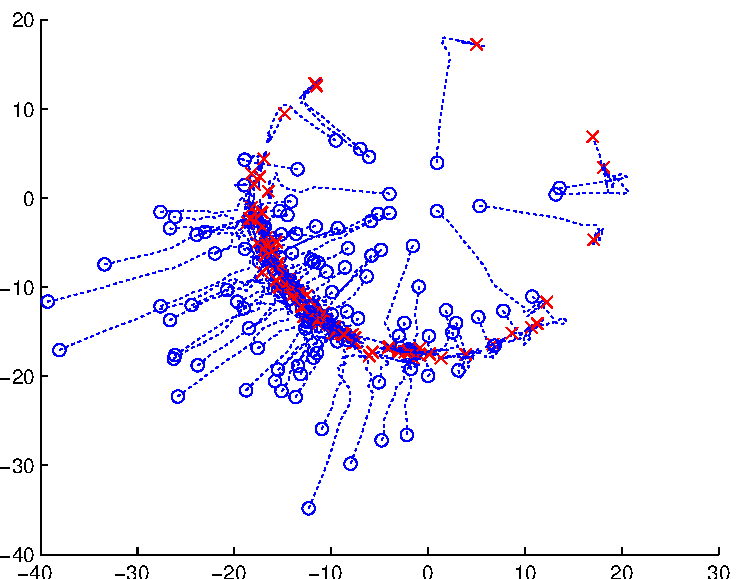
\includegraphics[width=0.45\columnwidth]{nlng_example_frame.pdf}
\caption{An example of the stochastic CPPF particle motion running on the multivariate benchmark model, showing $2$ of $10$ state dimensions. Prior states are shown with circles and posterior states with crosses.}
\label{fig:nlng_example_frame}
\end{figure}



\subsection{A Difficult Tracking Problem}

Now to a more applied problem. We consider tracking a small aircraft over a mapped landscape. Time of flight and doppler measurements from a radio transmitter on the aircraft provide accurate measurements of range $\rng{\rt}$, and range rate $\rng{\rt}$, but only a low resolution measurement of bearing $\bng{\rt}$. In addition, accurate measurements are made of the height above the ground $\hei{\rt}$. The profile of the terrain (i.e. the height of the ground above a datum at each point) has been mapped.

At $\rt$, the latent state for our model is,
%
\begin{IEEEeqnarray}{rCl}
 \ls{\rt} & = & \begin{bmatrix} \pos{\rt} \\ \vel{\rt} \end{bmatrix} \nonumber      ,
\end{IEEEeqnarray}
%
where $\pos{\rt}$ and $\vel{\rt}$ are the $3$-dimensional position and velocity of the aircraft respectively, and the observation is,
%
\begin{IEEEeqnarray}{rCl}
 \ob{\rt} & = & \begin{bmatrix} \bng{\rt} \\ \rng{\rt} \\ \hei{\rt} \\ \rngrt{\rt} \end{bmatrix}       .
\end{IEEEeqnarray}
%
The observation function is described by the following equations,
%
\begin{IEEEeqnarray}{rCl}
 \bng{\rt}   & = & \arctan\left(\frac{\pos{\rt,1}}{\pos{\rt,2}}\right) \nonumber \\
 \rng{\rt}   & = & \sqrt{ \pos{\rt,1}^2 + \pos{\rt,3}^2 + \pos{\rt,3}^2 } \nonumber \\
 \hei{\rt}   & = & \pos{\rt,3} - \terrain( \pos{\rt,1}, \pos{\rt,2} ) \nonumber \\
 \rngrt{\rt} & = & \frac{ \pos{\rt}\cdot\vel{\rt} }{ \rng{\rt} } \nonumber      ,
\end{IEEEeqnarray}
%
where $\terrain( \pos{\rt,1}, \pos{\rt,2} )$ is the terrain height at the corresponding horizontal coordinates. The four measurements are independent and the respective variances are $\left(\frac{\pi}{9}\right)^2$, $0.1^2$, $0.1^2$, $0.1^2$.

Two linear transition models have been used, both based on a near-constant velocity model, one with a Gaussian density and one with a Student-t density with $\dof = 3$ degrees of freedom,
%
\begin{IEEEeqnarray}{rCl}
 \transfun_1(\ls{\rt} | \ls{\rt-1}) & = & \normal{\ls{\rt}}{\transmat\ls{\rt-1}}{\transcov} \nonumber \\
 \transfun_2(\ls{\rt} | \ls{\rt-1}) & = & \studentt{\ls{\rt}}{\transmat\ls{\rt-1}}{\transcov}{\dof} \nonumber      ,
\end{IEEEeqnarray}
%
\begin{IEEEeqnarray}{rCl}
 \transmat & = & \begin{bmatrix} I & I \\ 0 & I \end{bmatrix} \nonumber \\
 \transcov & = & 10 \begin{bmatrix} \frac{1}{3} I & \frac{1}{2} I \\ \frac{1}{2} I &\ I \end{bmatrix} \nonumber \\
\end{IEEEeqnarray}

The accurate measurements of range, range rate and height constrain the region of high posterior probability to lie on a $3$ dimensional subspace, which can take some unusual shapes (see figure~\ref{fig:drone_example_frame}). This again means that particle filters using extended or unscented Kalman-type importance densities do not perform well. Furthermore, the optimal Gaussian importance density method performs particularly poorly as the maximisation procedure struggles with the narrow mode. For the simulations presented here, the terrain profile was modelled as a mixture of randomly-generated Gaussian blobs. An example is shown in figure~\ref{fig:drone_terrain_map}.
%
\begin{figure}
\centering
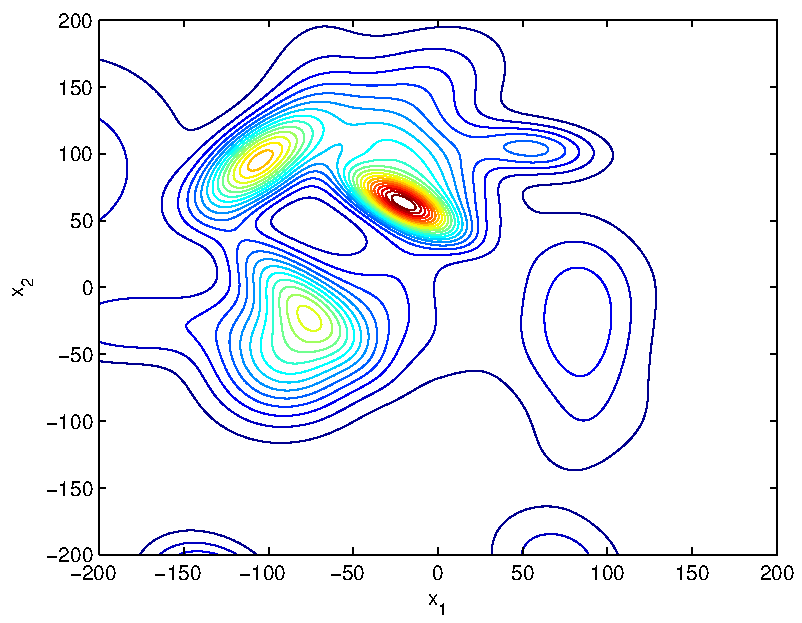
\includegraphics[width=0.45\columnwidth]{drone_terrain_map.pdf}
\caption{Contour plot of an example simulated terrain map.}
\label{fig:drone_terrain_map}
\end{figure}

The following particle filters were tested on the terrain tracking model:
\begin{itemize}
  \item A bootstrap particle filter
  \item A particle filter using an unscented Kalman-type importance density
  \item An optimal Gaussian importance particle filter
  \item A deterministic composite proposal particle filter with $\lgexpsf=0$
\end{itemize}

The number of particles used by each algorithm was selected so that the running times were roughly equal. The CPPF used in the region of $5$ to $10$ state updates per time step. For the student-t transition density, the CPPF uses the scale mixture of normals method.

Figure~\ref{fig:drone_example_frame} shows the motion of the particles from the stochastic CPPF on a typical frame, and the awkward shape of the posterior mode.% Figure~\ref{} shows the effective sample sizes of the particle approximations over a typical run with the Gaussian transition density.
%
\begin{figure}
\centering
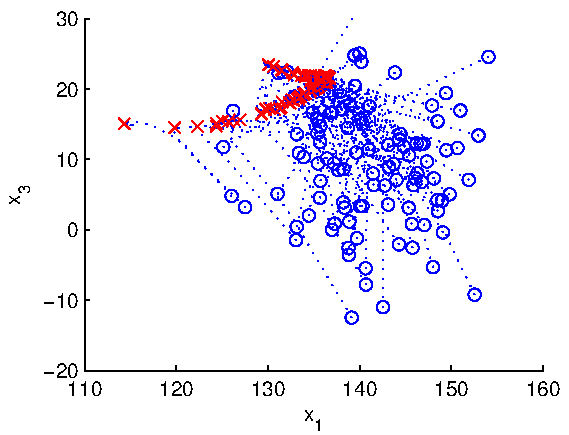
\includegraphics[width=0.45\columnwidth]{drone_example_frame.pdf}
\caption{An example of the stochastic CPPF particle motion running on the terrain tracking model, showing one horizontal and the vertical state component. Prior states are shown with circles and posterior states with crosses.}
\label{fig:drone_example_frame}
\end{figure}

A stochastic CPPF using resample-move was also tested, with the number of particles adjusted for a roughly-equal running time. This obtained almost identical average RMSEs to the deterministic CPPF, but higher effective sample sizes (but of course, with increased dependence between particles). Using $\lgexpsf=0.3$, roughly $25$--$50\%$ of the MH steps were accepted at each time step.

Table~\ref{tab:drone_results_gaussian} shows the average ESSs and RMSEs for each algorithm over 100 simulated data sets, each of 100 time steps using the Gaussian transition density. The same is shown for the student-t transition density in table~\ref{tab:drone_results_studentt}.
%
\begin{table}
\centering
\begin{tabular}{l||c|c|c}
Algorithm                                & $N_F$ & ESS  & RMSE \\
\hline
Bootstrap                                &  6000 &  1.0 & 78.6 \\
Unscented Kalman Proposal                &   460 &  2.4 & 70.2 \\
Optimal Gaussian Proposal                &    10 &  3.1 & 62.9 \\
Deterministic Composite Proposal         &   180 & 56.4 & 22.3 \\
\end{tabular}
\caption{Algorithm performance results on the terrain tracking model with Gaussian innovations.}
\label{tab:drone_results_gaussian}
\end{table}
%
\begin{table}
\centering
\begin{tabular}{l||c|c|c}
Algorithm                                & $N_F$ & ESS  & RMSE \\
\hline
Bootstrap                                &  6000 &  1.0 & 133.7 \\
Unscented Kalman Proposal                &   460 &  3.4 & 110.3 \\
Optimal Gaussian Proposal                &    10 &  2.9 & 105.1 \\
Deterministic Composite Proposal         &   180 & 17.2 & 48.0 \\
\end{tabular}
\caption{Algorithm performance results on the terrain tracking model with student-t innovations.}
\label{tab:drone_results_studentt}
\end{table}

It was found that as $\dof$ is decreased, the performance of the composite proposal particle filter deteriorated relative to the simpler algorithms, with the average ESS falling to around $6.0$ when $\dof=1$ (i.e. when the transition model has a Cauchy distribution). This is unsurprising, given that the scale of outliers increases as $\dof$ decreases.



\subsection{A Heartbeat Inference Problem}

As a final example, we consider the problem of detecting heartbeats in a vibration signal. Measurements from an accelerometer are first partitioned into segments believed to contain a heartbeat, and a particle filter is then used to infer its properties. The $t$th heartbeat is modelled parametrically as the product of a Gaussian envelope with amplitude $\amp{\rt}$ and width $\wid{\rt}$, and a sine wave carrier with frequency $\freq{\rt}$ and relative phase $\pha{\rt}$. The time shift of the centre of the heartbeat within the measurement is $\del{\rt}$, and the sensor exhibits a D.C. bias $\bias{\rt}$ which varies slowly over time. The resulting observation function is highly nonlinear, with the $d$th component given by,
%
\begin{IEEEeqnarray}{rCl}
 \obsfun(\ls{\rt})_d & = & \amp{\rt} \exp\left\{ -\frac{ (T\,d - \del{\rt})^2 }{ 2\wid{\rt}^2 } \right\} \sin\left( \freq{\rt}(T\,d - \del{\rt}) + \pha{\rt} \right) + \bias{\rt} \nonumber      ,
\end{IEEEeqnarray}
%
where $T$ is the sampling period of the sensor. Each observation consists of $50$ time samples and the observation density is modelled as a Gaussian with a covariance matrix $0.2^2 I$. An example heartbeat simulated from this model is shown in figure~\ref{fig:sineha_example_beat}.
%
\begin{figure}
\centering
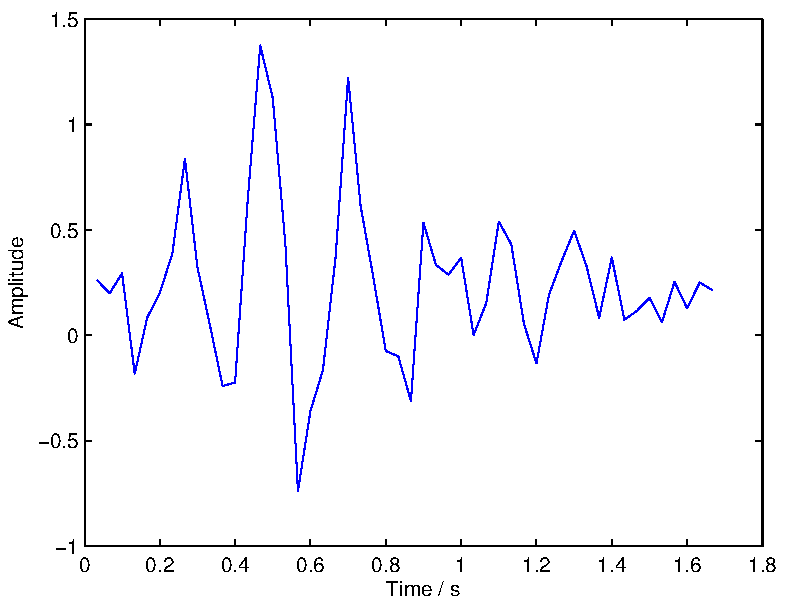
\includegraphics[width=0.45\columnwidth]{sineha_example_beat.pdf}
\caption{An example heartbeat simulated from the model.}
\label{fig:sineha_example_beat}
\end{figure}

The latent state is,
%
\begin{IEEEeqnarray}{rCl}
 \ls{\rt} & = & \begin{bmatrix} \amp{\rt} & \wid{\rt} & \del{\rt} & \freq{\rt} & \pha{\rt} & \bias{\rt} \end{bmatrix}^T      .
\end{IEEEeqnarray}
%
The transition density is factorised into independent terms, with $\freq{\rt}$, $\pha{\rt}$ and $\bias{\rt}$ evolving according to a Gaussian random walk, and $\wid{\rt}$ according to a geometric random walk (i.e. with a log-normal density), while $\del{\rt}$ and $\amp{\rt}$ are gamma distributed with no dependence on their past values.
%
%\begin{IEEEeqnarray}{rCl}
% p(\amp{\rt} )                & = & \gammaden{\amp{\rt}-0.5}{10}{0.05} \nonumber \\
% p(\wid{\rt} | \wid{\rt-1})   & = & \lognormal{\wid{\rt}}{}{} \nonumber \\
% p(\del{\rt})                 & = &   \nonumber \\
% p(\freq{\rt} | \freq{\rt-1}) & = &   \nonumber \\
% p(\pha{\rt} | \pha{\rt-1})   & = &   \nonumber \\
% p(\bias{\rt} | \bias{\rt-1}) & = &   \nonumber      ,
%\end{IEEEeqnarray}
%%
%where {\meta PARAMETERS}.

The complications introduced in the posterior distribution by the highly multi-modal observation density mean that simple Gaussian importance densities do not work very well. Particle filters using extended or unscented Kalman-type importance densities fail immediately on this model.

The following particle filters were tested on the heartbeat inference model:
\begin{itemize}
  \item A bootstrap particle filter
  \item An optimal Gaussian importance particle filter
  \item A deterministic composite proposal particle filter with $\lgexpsf=0$
\end{itemize}

The number of particles used by each algorithm was selected so that the running times were roughly equal. In order to use a CPPF with this model, the OID density sequence must be approximated with Gaussians. This is achieved by linearising the observation model around the current state \eqref{eg:linearised_Gaussian_approx} and using the log-density Taylor series truncation method for the prior \eqref{eg:general_Gaussian_approx}. The variance terms in this latter approximation are limited to be no greater than the prior variances. The CPPF uses the adaptive step size method and made in the region of $5$ to $15$ state updates per time step, with the exception of a few particles which tended to ``get stuck'' and were discarded after 50 steps.

Figure~\ref{fig:sineha_example_frame} shows the motion of the particles from the deterministic CPPF on a typical frame. Table~\ref{tab:sineha_results} shows the average ESSs and RMSEs for each algorithm over 100 simulated data sets, each of 100 time steps.%Figure~\ref{} shows the effective sample sizes of the particle approximations over a typical run.
%
\begin{table}
\centering
\begin{tabular}{l||c|c|c}
Algorithm                                & $N_F$ & ESS  & RMSE \\
\hline
Bootstrap                                & 15000 &  7.6 &  2.0 \\
Optimal Gaussian Proposal                &   200 &  8.8 &  2.0 \\
Deterministic Composite Proposal         &   800 & 72.8 &  1.4 \\
\end{tabular}
\caption{Algorithm performance results on the heartbeat inference model.}
\label{tab:sineha_results}
\end{table}
%
\begin{figure}
\centering
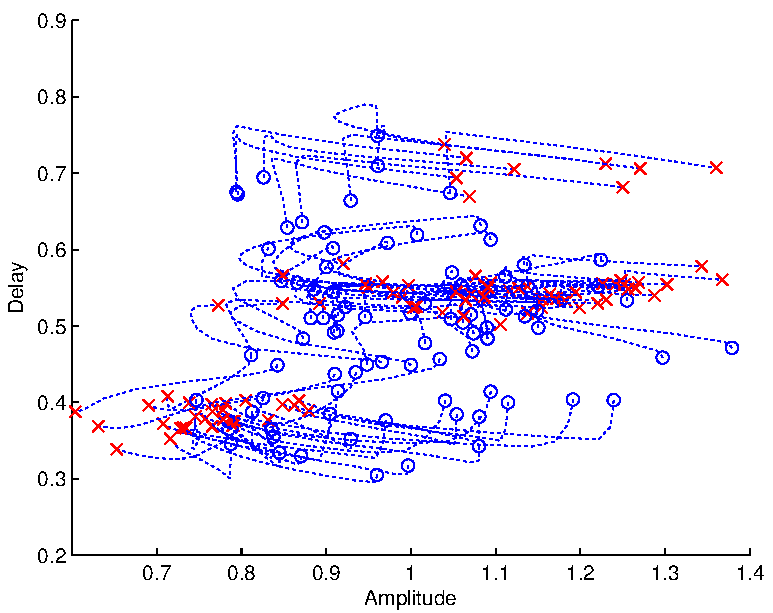
\includegraphics[width=0.45\columnwidth]{sineha_example_frame.pdf}
\caption{An example of the S-CPPF particle motion running on the heartbeat inference model, showing amplitude and delay state components. Prior states are shown with circles and posterior states with crosses.}
\label{fig:sineha_example_frame}
\end{figure}



\section{Conclusions}

We have detailed a new mechanism for conducting the update state in a particle filter, the composite proposal method. This works by introducing the effect of the observation progressively and adjusting the particle state incrementally so as to achieve a better distribution.

The simulations presented in the previous section demonstrate that the composite proposal procedure is capable of achieving better particle approximations (i.e. higher effective sample sizes) than simpler particle filters (which use a single Gaussian importance density) on a class of challenging state space models. Furthermore, the particles thus generated are independent conditional on the resampled particle set from the preceding time step, a property not achieved by filters using annealing or resample-move.

The models for which the composite proposal particle filter appears most effective are those with Gaussian transition and observation densities but highly nonlinear transition and observation functions. For this class, the performance improvement relative to the simpler algorithms with an equal processing time is very great. Moreover, the requisite Gaussian approximation is ``obvious'', simply a linearisation of the observation function, meaning that the algorithm requires almost no tuning (the tolerance for the adaptive step-size selection process is the only critical parameter).

With non-Gaussian model densities, the performance gains from the composite proposal particle filter are more modest, both when using the scale mixture of normals method and Gaussian approximations formed by linearisation of the log of the optimal importance density. In addition, when more drastic approximations are required, a greater degree of algorithm tuning is required, such as limiting the variance of the approximation to prevent instability.

In general, there is no guarantee that the CPPF will outperform any other particle filter, not even a bootstrap filter. Indeed pathological examples may be constructed on which it will be inferior to the competition. However, the same may be said of all existing particle filters. The choice of the right algorithm will often require a comparison on the particular application being studied.



\section{THINGS TO DO}
\begin{itemize}
  \item Revise Numerical simulations.
\end{itemize}



\appendix

\section{Appropriate Dynamics Leading to a Standard Gaussian Stationary Distribution} \label{app:stationary_ou_process}

By using a Gaussian approximation, appropriate state update formulas may be derived by consideration of an underlying standard Gaussian variable,
%
\begin{IEEEeqnarray}{rCl}
 \ls{\pt} & = & \lgoimean{\pt} + \lgoicov{\pt}^{\half} \stdnorm{\pt} \nonumber \\ \\
 \stdnorm{\pt} & \sim & \normal{\stdnorm{\pt}}{0}{I} \nonumber      .
\end{IEEEeqnarray}

There is an infinitude of possible dynamical systems which maintain the correct marginal distribution. We narrow this down with the pragmatic approach that the system should be analytically integrable. Such is the case for a stationary Ornstein-Uhlenbeck process governed by,
%
\begin{IEEEeqnarray}{rCl}
 d\stdnorm{\pt} & = & \oudrift{} \stdnorm{\pt} d\pt + \oudiffuse{} d\lginfbm{\pt} \nonumber      ,
\end{IEEEeqnarray}
%
subject to $\oudiffuse{\pt}\oudiffuse{\pt}^T = \oudrift{\pt}+\oudrift{\pt}^T$. The condition arises from writing the variance a short time in the future,
%
\begin{IEEEeqnarray}{rCl}
 \variance{}\left[\stdnorm{\pt+\dpt}\right] & = & \variance{}\left[ \stdnorm{\pt} - \oudrift{} \stdnorm{\pt} \dpt + \oudiffuse{} \delta\lginfbm{\pt} + \bigo{\dpt^2} \right] \nonumber \\
 & = & \variance{}\left[ \left(I-\dpt\oudrift{}\right) \stdnorm{\pt} \right] + \variance{}\left[ \oudiffuse{} \delta \lginfbm{\pt} \right] + \variance{}\left[ \bigo{\dpt^2} \right] \nonumber \\
 & = & I + \dpt\left[\oudiffuse{\pt}\oudiffuse{\pt}^T - \left(\oudrift{\pt}+\oudrift{\pt}^T\right)\right] + \bigo{\dpt^2} \nonumber      .
\end{IEEEeqnarray}

Next consider the form of $\oudrift{}$. In order to avoid arbitrary biases in a particular direction of $\stdnorm{\pt}$, this matrix should be diagonal. Finally, since the increments $d\lginfbm{\pt}$ are independent and rotating does not affect their distribution, $\oudiffuse{\pt}$ may be made positive semidefinite without loss of generality, and hence must also be diagonal. Together, these conditions leave us with the following stochastic differential equation (SDE),
%
\begin{IEEEeqnarray}{rCl}
 d\stdnorm{\pt} & = & -\half \lgexpsf \stdnorm{\pt} d\pt + \lgexpsf^{\half} d\lginfbm{\pt} \nonumber      .
\end{IEEEeqnarray}

To integrate this SDE, observe that,
%
\begin{IEEEeqnarray}{rCl}
 d\left[\exp\left\{\half\lgexpsf\pt\right\}\stdnorm{\pt}\right] & = & \half \lgexpsf \exp\left\{\half\lgexpsf\pt\right\}\stdnorm{\pt} d\pt + \exp\left\{\half\lgexpsf\pt\right\} d\stdnorm{\pt} \nonumber \\
 & = & \lgexpsf^{\half} d\lginfbm{\pt} \nonumber      .
\end{IEEEeqnarray}
%
Hence,
%
\begin{IEEEeqnarray}{rCl}
 \exp\left\{\half\lgexpsf\pt_1\right\} \stdnorm{\pt_1} - \exp\left\{\half\lgexpsf\pt_0\right\} \stdnorm{\pt_0} & = & (\pt_1-\pt_0) \lgexpsf^{\half} \stdnorm{\Delta} \nonumber      ,
\end{IEEEeqnarray}
%
so,
%
\begin{IEEEeqnarray}{rCl}
 \stdnorm{\pt_1} & = & \exp\left\{ -\half \lgexpsf (\pt_1-\pt_0) \right\} \stdnorm{\pt_0} + \left[ 1 - \exp\left\{ - \lgexpsf (\pt_1-\pt_0) \right\} \right]^{\half} \stdnorm{\Delta} \nonumber       .
\end{IEEEeqnarray}



\section{A Stochastic Differential Equation For State Evolution} \label{app:state_SDE}

For clarity, write $\lgoimean{\pt}$ instead of $\lgoimeanapprox{\pt}{\ls{\pt_0}}$ and $\lgoicov{\pt}$ instead of $\lgoicovapprox{\pt}{\ls{\pt_0}}$ throughout this proof.

The state $\ls{\pt}$ is a modelled as linear transformation of an underlying standard Gaussian random variable,
%
\begin{IEEEeqnarray}{rCl}
 \ls{\pt} & = & \lgoimean{\pt} + \lgoicov{\pt}^{\half} \stdnorm{\pt} \label{app-eq:gaussian_decomposition} \\
 \stdnorm{\pt} & \sim & \normal{\stdnorm{\pt}}{0}{I} \nonumber      .
\end{IEEEeqnarray}

This underlying variable is made to vary according to a stationary Ornstein-Uhlenbeck process,
%
\begin{IEEEeqnarray}{rCl}
 d\stdnorm{\pt} & = & -\half \lgexpsf \stdnorm{\pt} d\pt + \lgexpsf^{\half} d\lginfbm{\pt} \label{app-eq:standard_normal_SDE}      .
\end{IEEEeqnarray}

Differentiating \eqref{app-eq:gaussian_decomposition} and substituting \eqref{app-eq:standard_normal_SDE},
%
\begin{IEEEeqnarray}{rCl}
 d\ls{\pt} & = & \frac{\partial \lgoimean{\pt}}{\partial \pt} d\pt + \half \frac{\partial \lgoicov{\pt} }{\partial \pt} \lgoicov{\pt}^{-\half} \stdnorm{\pt} d\pt + \lgoicov{\pt}^{\half} d\stdnorm{\pt} \nonumber \\
 & = & \frac{\partial \lgoimean{\pt}}{\partial \pt} d\pt + \half \frac{\partial \lgoicov{\pt} }{\partial \pt} \lgoicov{\pt}^{-\half} \left(\ls{\pt}-\lgoimean{\pt}\right) d\pt \nonumber \\
 &   & \qquad \qquad + \: \lgoicov{\pt}^{\half} \left[ -\half \lgexpsf \left(\ls{\pt}-\lgoimean{\pt}\right) d\pt + \lgexpsf^{\half} d\lginfbm{\pt} \right] \nonumber \\
 & = & \left[ \frac{\partial \lgoimean{\pt}}{\partial \pt} + \half \left( \frac{\partial \lgoicov{\pt} }{\partial \pt} \lgoicov{\pt}^{-1} - \lgexpsf I \right) (\ls{\pt}-\lgoimean{\pt}) \right] d\pt + \lgexpsf^{\half} \lgoicov{\pt}^{\half} d\lginfbm{\pt}      .
\end{IEEEeqnarray}

In the partially linear-Gaussian case, or when the Gaussian OID approximation takes the following form,
%
\begin{IEEEeqnarray}{rCl}
 \lgoicov{\pt} & = & \left[ \transcov^{-1} + \pt \obsmat^T \obscov^{-1} \obsmat \right]^{-1} \nonumber \\
 \lgoimean{\pt}    & = & \lgoicov{\pt} \left[ \transcov^{-1} \transfun(\ls{\rt-1}) + \pt \obsmat^T \obscov^{-1} \ob{\rt} \right] \nonumber     ,
\end{IEEEeqnarray}
%
then
%
\begin{IEEEeqnarray}{rCl}
 \frac{\partial \lgoicov{\pt} }{\partial \pt} & = & -\lgoicov{\pt} \obsmat^T \obscov^{-1} \obsmat \lgoicov{\pt} \nonumber \\
 \frac{\partial \lgoimean{\pt}}{\partial \pt} & = & \lgoicov{\pt} \obsmat^T \obscov^{-1}(\ob{\rt}-\obsmat\lgoimean{\pt}) \nonumber       ,
\end{IEEEeqnarray}
%
and the state evolution stochastic differential equation becomes,
%
\begin{IEEEeqnarray}{rCl}
 d\ls{\pt} & = & \left[ \lgoicov{\pt} \obsmat^T \obscov^{-1} \left( (\ob{\rt}-\obsmat\lgoimean{\pt}) - \half \obsmat (\ls{\pt}-\lgoimean{\pt}) \right) - \half \lgexpsf (\ls{\pt}-\lgoimean{\pt}) \right] d\pt + \lgexpsf^{\half} \lgoicov{\pt}^{\half} d\lginfbm{\pt} \nonumber       .
\end{IEEEeqnarray}

\section{Governing Equation Optimal Particle Transport} \label{app:optimal_flow_governing_eq}

This exposition is based closely on that of \cite{Daum2008}, but we consider moving each particle according to its OID sequence rather than the filtering distribution. We omit the time subscripts, particle superscripts and the dependence on $\ls{\rt-1}$ for clarity. In addition, write the following shorthands,
%
\begin{IEEEeqnarray}{rCl}
 \logtrans(\ls{}) & = & \log\left(\transden(\ls{\rt}|\ls{\rt-1})\right) \nonumber \\
 \logobs(\ls{}) & = & \log\left(\obsden(\ob{\rt}|\ls{\rt})\right) \nonumber \\
 \logoiden{\pt}(\ls{\pt}) & = & \log\left( \oiden{\pt}(\ls{\pt}) \right) \nonumber       .
\end{IEEEeqnarray}

An equation for the optimal flow may be derived by considering the sequence of densities, $\oiden{\pt}(\ls{\pt})$. Taking the log and differentiating with respect to $\pt$ and $\ls{\pt}$,
%
\begin{IEEEeqnarray}{rCl}
 \logoiden{\pt}(\ls{\pt}) & = & \logtrans(\ls{\pt}) + \pt \logobs(\ls{\pt}) - \log\left(\oinorm{\pt}\right)     ,
\end{IEEEeqnarray}
%
\begin{IEEEeqnarray}{rCl}
 \frac{\partial \logoiden{\pt}}{\partial \pt} & = & \frac{ 1 }{ \oiden{\pt}(\ls{\pt}) } \frac{\partial \oiden{\pt}}{\partial \pt} \nonumber \\
  & = & \logobs(\ls{\pt}) - \frac{d}{d\pt}\log\left(\oinorm{\pt}\right) \label{eq:dpi-dlam}     ,
\end{IEEEeqnarray}
%
\begin{IEEEeqnarray}{rCl}
 \frac{\partial \logoiden{\pt}}{\partial \ls{\pt}} & = & \frac{ 1 }{ \oiden{\pt}(\ls{\pt}) } \frac{\partial \oiden{\pt}}{\partial \ls{\pt}} \label{eq:dpi-dx}     .
\end{IEEEeqnarray}
%
\begin{IEEEeqnarray}{rCl}
 \frac{\partial^2 \logoiden{\pt}}{\partial \ls{\pt}^2} & = & \frac{ \oiden{\pt}(\ls{\pt}) \frac{\partial^2 \oiden{\pt}}{\partial \ls{\pt}^2} - \frac{\partial \oiden{\pt}}{\partial \ls{\pt}}\frac{\partial \oiden{\pt}}{\partial \ls{\pt}}^T }{ \oiden{\pt}(\ls{\pt})^2 } \nonumber \\
 & = & \frac{ 1 }{ \oiden{\pt}(\ls{\pt}) } \frac{\partial^2 \oiden{\pt}}{\partial \ls{\pt}^2} - \frac{\partial \logoiden{\pt}}{\partial \ls{\pt}}\frac{\partial \logoiden{\pt}}{\partial \ls{\pt}}^T \label{eq:d2pi-dx2}     .
\end{IEEEeqnarray}
%
Also,
%
\begin{IEEEeqnarray}{rCl}
 \frac{d}{d\pt}\log\left(\oinorm{\pt}\right) & = & \frac{\frac{d\oinorm{\pt}}{d\pt}}{\oinorm{\pt}} \nonumber \\
                                               & = & \frac{ \int \transden(\ls{\rt}|\ls{\rt-1}) \obsden(\ob{\rt}|\ls{\rt})^\pt \logobs(\ls{}) d\ls{\rt} }{ \int \transden(\ls{\rt}|\ls{\rt-1}) \obsden(\ob{\rt}|\ls{\rt})^\pt d\ls{\pt} } \nonumber \\
                                               & = & \expect{\oiden{\pt}}\left[ \logobs(\ls{}) \right]     .
\end{IEEEeqnarray}

The Fokker-Planck equation relates the flow of a particle with the evolution of the density for its position. For a particle moving according to,
%
\begin{IEEEeqnarray}{rCl}
 d\ls{\pt} & = & \flowdrift{\pt}(\ls{\pt}) d\pt + \flowdiffuse{\pt} d\flowbm{\pt}     ,
\end{IEEEeqnarray}
%
Fokker-Planck then states,
%
\begin{IEEEeqnarray}{rCl}
 \frac{\partial \oiden{\pt}}{\partial \pt} & = & - \nabla \cdot \left[ \flowdrift{\pt}(\ls{\pt}) \oiden{\pt}(\ls{\pt}) \right] + \nabla \cdot \left[ \flowcov{\pt} \nabla \oiden{\pt}(\ls{\pt}) \right] \nonumber \\
 & = & - \trace\left[ \frac{\partial}{\partial \ls{\pt}} \left( \flowdrift{\pt}(\ls{\pt}) \oiden{\pt}(\ls{\pt}) \right) \right] + \trace\left[ \frac{\partial}{\partial \ls{\pt}} \left( \flowcov{\pt} \frac{\partial \oiden{\pt}}{\partial \ls{\pt}} \right) \right] \nonumber      ,
\end{IEEEeqnarray}
%
where,
%
\begin{IEEEeqnarray}{rCl}
 \flowcov{\pt} & = & \frac{1}{2} \flowdiffuse{\pt} \flowdiffuse{\pt}^T \nonumber      .
\end{IEEEeqnarray}
%
Expanding and substituting the preceding intermediate results, we have,
%
\begin{IEEEeqnarray}{rCl}
 \frac{\partial \oiden{\pt}}{\partial \pt} & = & -\trace\left[ \oiden{\pt}(\ls{\pt}) \frac{\partial \flowdrift{\pt}}{\partial \ls{\pt}} + \flowdrift{\pt}(\ls{\pt})^T \frac{\partial \oiden{\pt}}{\partial \ls{\pt}} \right] + \trace\left[ \flowcov{\pt} \frac{\partial^2 \oiden{\pt}}{\partial \ls{\pt}^2} \right] \nonumber \\
 \oiden{\pt}(\ls{\pt}) \left[ \logobs(\ls{}) - \frac{d}{d\pt}\log\left(\oinorm{\pt}\right) \right] & = & -\trace\left[ \oiden{\pt}(\ls{\pt}) \frac{\partial \flowdrift{\pt}}{\partial \ls{\pt}} + \oiden{\pt}(\ls{\pt}) \flowdrift{\pt}(\ls{\pt})^T \frac{\partial \logoiden{\pt}}{\partial \ls{\pt}} \right] \nonumber \\
 & & \qquad + \: \trace\left[ \flowcov{\pt} \oiden{\pt}(\ls{\pt}) \left( \frac{\partial^2 \logoiden{\pt}}{\partial \ls{\pt}^2} + \frac{\partial \logoiden{\pt}}{\partial \ls{\pt}}\frac{\partial \logoiden{\pt}}{\partial \ls{\pt}}^T \right)\right] \nonumber \\
 \logobs(\ls{}) - \expect{\oiden{\pt}}\left[ \logobs(\ls{}) \right] & = & -\trace\left[ \frac{\partial \flowdrift{\pt}}{\partial \ls{\pt}} \right] - \flowdrift{\pt}(\ls{\pt})^T \frac{\partial \logoiden{\pt}}{\partial \ls{\pt}} \nonumber \\
 & & \qquad + \: \trace\left[ \flowcov{\pt} \left(\frac{\partial^2 \logoiden{\pt}}{\partial \ls{\pt}^2} \right) \right] + \frac{\partial \logoiden{\pt}}{\partial \ls{\pt}}^T \flowcov{\pt} \frac{\partial \logoiden{\pt}}{\partial \ls{\pt}} \nonumber      ,
\end{IEEEeqnarray}
%
where $\frac{\partial \flowdrift{\pt}}{\partial \ls{\pt}}$ is the Jacobian of the drift and $\frac{\partial \logoiden{\pt}}{\partial \ls{\pt}}$ and $\frac{\partial^2 \logoiden{\pt}}{\partial \ls{\pt}^2}$ are the gradient and Hessian of the log-density respectively, and where in the last step we have divided through by $\oiden{\pt}$. This requires the density to be nowhere vanishing. The result is a partial differential equation, for which any solution, $\flowdrift{\pt}$ and $\flowdiffuse{\pt}$, will produce an optimal flow, distributed according to $\oiden{\pt}$ throughout.



\bibliographystyle{chicago}
\bibliography{D:/pb404/Dropbox/PhD/OTbib}
%\bibliography{/home/pete/Dropbox/PhD/OTbib}

\end{document} 